\documentclass{article}
\usepackage[utf8]{inputenc}
\usepackage{lmodern}
\usepackage[T1]{fontenc}
\usepackage[utf8]{inputenc}
\usepackage[spanish,activeacute]{babel}
\usepackage{titlesec}
\usepackage[obeyspaces]{url}
\usepackage[a4paper, margin=1in]{geometry}
\titleformat{\section}
  {\normalfont\fontsize{14}{14}\bfseries}{\thesection}{1em}{}
\titlespacing{\paragraph}{0pt}{1.5em}{.5em}[]
\titleformat{\paragraph}
{\normalfont\normalsize\bfseries}{\theparagraph}{1em}{}
\titlespacing*{\paragraph}
{0pt}{3.25ex plus 1ex minus .2ex}{1.5ex plus .2ex}
\inputencoding{utf8}
\usepackage{mathtools}
\usepackage{graphicx}
\DeclareGraphicsExtensions{.png,.pdf,.jpg,.webp}
\usepackage{float}
\usepackage{amssymb}
\usepackage{cancel}
\usepackage{bm}
\usepackage{amsmath}
\usepackage{color}
\usepackage{caption}
\usepackage[colorlinks=true,linkcolor=blue]{hyperref}%
\usepackage[toc,title,page]{appendix}
\addto\captionsspanish{%
  \renewcommand\appendixname{Anexo}
  \renewcommand\appendixpagename{Anexos}
  \renewcommand\appendixtocname{Anexos}
}
\usepackage{listingsutf8}
\usepackage{listings}
\renewcommand{\lstlistingname}{Código}
\renewcommand\lstlistlistingname{Códigos fuente}
\definecolor{dkgreen}{rgb}{0,0.6,0}
\definecolor{ltgray}{rgb}{0.5,0.5,0.5}
\hypersetup{
    colorlinks,
    citecolor=black,
    filecolor=black,
    urlcolor=black
}


\title{Taller de Coches}
\author{Martin Fagoaga y Gonzalo Álvarez}
\date{2022}
\begin{document}
\maketitle 
\begin{figure}[H]
  \centering
  \includegraphics[width=1.0\textwidth]{pexels-cottonbro-4480505.jpg}
\end{figure}
\clearpage

{
  \hypersetup{ linkcolor=black}
  \tableofcontents
\clearpage
\listoffigures
\clearpage
\clearpage
\lstlistoflistings
\clearpage
}

\section{FASE 1: ANALISIS Y DISEÑO}
\subsection{Introducción: AppTaller}
\subsection{Objetivos}
\subsection{Contextualización del proyecto}
\subsection{Análisis}
\subsection{Diseño} 
\subsection{Planificación semanal}
\subsection{FOL}
\section{FASE 2: IMPLEMENTACIÓN Y PRUEBAS}
{
  \lstset{%
  	backgroundcolor=\color{white},
      inputencoding=utf8,
    escapeinside={\%*}{*)},
    literate={á}{{\'a}}1 {é}{{\'e}}1 {í}{{\'i}}1 {ó}{{\'o}}1 {ú}{{\'u}}1 {Á}{{\'A}}1 {É}{{\'E}}1 {Í}{{\'I}}1 {Ó}{{\'O}}1 {Ú}{{\'U}}1 {ñ}{{\~n}}1 {Ñ}{{\~N}}1,
  	basicstyle=\footnotesize,
  	breakatwhitespace=false,
  	breaklines=true,
    nolol=true,
  	captionpos=b,
  	commentstyle=\color{dkgreen},
  	deletekeywords={...},
  	escapeinside={\%*}{*)},
  	extendedchars=true,
  	frame=single,
  	keepspaces=true,
  	keywordstyle=\color{blue},
  	language=SQL,
  	morekeywords={*,modify,MODIFY,...},
  	numbers=left,
  	numbersep=15pt,
  	numberstyle=\tiny,
  	rulecolor=\color{ltgray},
  	showspaces=false,
  	showstringspaces=false, 
  	showtabs=false,
  	stepnumber=1,
  	tabsize=3,
}
\subsection{DDBB: Código SQL}
Para ver la instalación de la BBDD de oracle, referiros a la sección de Sistemas Informáticos, en este apartado nos limitaremos a describir el código sql ejecutado en la BD.\\
Para poner en marcha nuestra base de datos, primero hemos creado dos datafiles en los que se dividirá el contenido. \\ Luego hemos creado un usuario de jefe o administrador, y 5 cuentas para los mecánicos, y hemos modificado sus perfiles,
permitiendo tan solo 1 inicio de sesión simultaneo por usuario. También hemos creado un usuario para los visitantes de la web, este usuario tiene la posibilidad de crear sesiones simultaneas ilimitadas. \\ 
Luego hemos creado las tablas que podemos observar en los diagramas. Cabe destacar que para tener IDs autogenerados ascendentes, hemos utilizado la siguiente secuencia:\\
\begin{lstlisting}{sql}
  CREATE SEQUENCE CLIENTES_SEQ START WITH 1;

  CREATE OR REPLACE TRIGGER CLIENTES_IDS BEFORE INSERT ON CLIENTE FOR EACH ROW
  BEGIN SELECT CLIENTES_SEQ.NEXTVAL INTO :NEW.ID_CLIENTE FROM DUAL;
  END;
\end{lstlisting}
Después de crear las tablas hemos establecido las relaciones entre ellas y hemos añadido algún constraint como puede ser el formato de DNI de un cliente o el formato de un correo electrónico.\\ 
Hemos limitado los permisos que tienen los mecánicos en las tablas, ya que en nuestro diseño no deben ser capaces de modificar algunos parámetros como pueden ser los precios de las piezas. También hemos concedido permiso para
realizar select en las tablas de piezas y categorías al usuario de la web, ya que son las únicas tablas que debe ver, y en ningún caso editar.\\ 
Finalmente, hemos insertado datos de prueba en todas las tablas para comprobar la correcta creación de estas y tener una base sobre la que trabajar.\\ 
Todas las ordenes sql realizadas están en el script disponible en el Anexo \ref{appendix:BBDD}.
}

\subsection{Programación: Clases y métodos}
  En nuestro programa hemos decidido separar la lógica de negocio de las interfaces.\\ 
  Hemos dividido las clases en 4 paquetes:\\
  \begin{itemize}
    \item Modelos: En este paquete están las clases que representan las entidades del negocio. 
    \item DAO: En este paquete están las clases que se encargan de realizar la conexión con la base de datos, y realizar las querys necesarias.
    \item System: En este paquete están las clases que contienen los metodos que realizan las acciones relacionadas con el negocio, como buscar una factura concreta o crear una reparacion. En este paquete hemos creado una clase llamada CreadorPDF 
    que hace uso de la librería \href{https://github.com/itext}{\color{red}{iText}} para crear una factura en formato .pdf.
    \item UI: En este paquete están las interfaces gráficas con sus controladores. 
  \end{itemize}
  El código fuente de todo el programa se puede ver en el Anexo \ref{appendix:programacion}.

\subsection{Lenguaje de Marcas: conjunto de ficheros}
\subsection{SSII: Instalación y configuración y puesta en marcha.} 
\subsubsection{Hardware}
En nuestro caso hemos optado por equipar el taller con 4 portátiles con el SO Windows. 1 de ellos
estaría colocado en la oficina y será el portátil del administrador, los otros 3 estarán colocados 
en los puestos de reparación de vehículos del taller.\\ La conexión a internet se realizará via Wi-Fi, utilizando el Wi-Fi emitido por el router que estará en la oficina. Hemos optado 
por no utilizar cableado ya que creemos que hoy en día el Wi-Fi aporta suficiente fiabilidad y añadir cableado al taller podría provocar molestias a los empleados a la hora de utilizar 
maquinaría pesada y mover piezas por el taller.\\
Debido a las limitadas necesidades que tendrán estos portátiles, hemos optado por el modelo \href{https://www.pccomponentes.com/acer-travelmate-p2-tmp214-53-37at-intel-core-i3-1115g4-8gb-256gb-ssd-14}{\color{red}{{Acer Travelmate P2}}}.\\
\begin{figure}[H]
  \centering
  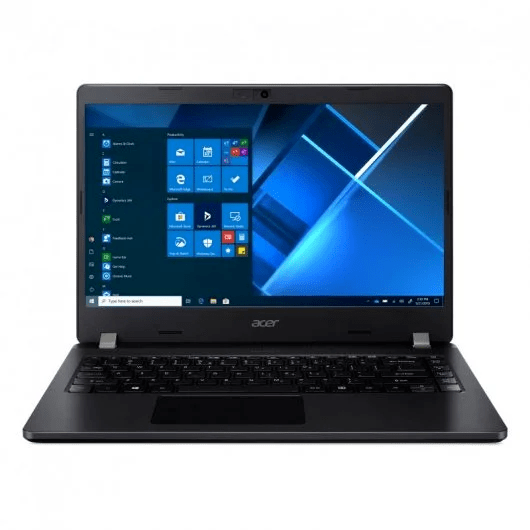
\includegraphics[width=0.6\textwidth]{CapturasSistemas/portatil.png}
  \caption{Portátil Acer Travelmate P2}
  \caption*{Fuente: \href{https://www.pccomponentes.com/acer-travelmate-p2-tmp214-53-37at-intel-core-i3-1115g4-8gb-256gb-ssd-14}{https://www.pccomponentes.com/}}
\end{figure}
\begin{itemize}
  \item Procesador: Intel Core i3-1115g4
  \item Memoria Ram: 8 GB DDR4
  \item Almacenamiento: 256 GB SSD PCIe
  \item Conectividad: \begin{itemize}
    \item Gigabit Ethernet
    \item Intel Wi-Fi 6 AX201 (802.11)
    \item Bluetooth
  \end{itemize}
  \item SO: Windows 10 Home 64 Bits
\end{itemize}
La base de datos y la página web la alojaremos en un VPS con una instalación del SO Ubuntu Server. En nuestro caso hemos optado por contratar el servidor \href{https://www.arsys.es/servidores/vps}{\color{red}{Arsys VPS M}},
ya que su centro de datos está en España, con lo que tendriamos una latencia más baja que con otras opciones. \\
Finalmente, para la línea telefónica y de internet hemos optado por contratar la operadora Guuk. Con una velocidad de 600mb simétricos, creemos que es suficiente para las necesidades del taller. \\

Presupuesto total de hardware/Software: \\
\begin{itemize}
  \item Portátiles: 1864.12€
  \item Servidor: 120€/Año
  \item Dominio: 15€/Año
  \item Internet: 504€/Año
\end{itemize}
\subsubsection{Software}
{
En los portátiles con Windows 10, instalariamos el programa AppTaller creado por nosotros. No haría falta nada más para tener los ordenadores operativos. \\ 
\paragraph{Instalación SGDB}
Para poner en marcha la base de datos en el servidor, primero hemos instalado docker en el mismo. Para ello hemos ejecutado los siguientes comandos: 
  \lstset{%
  	backgroundcolor=\color{white},
    inputencoding=utf8,
    language=bash,
    escapeinside={\%*}{*)},
    literate={á}{{\'a}}1 {é}{{\'e}}1 {í}{{\'i}}1 {ó}{{\'o}}1 {ú}{{\'u}}1 {Á}{{\'A}}1 {É}{{\'E}}1 {Í}{{\'I}}1 {Ó}{{\'O}}1 {Ú}{{\'U}}1 {ñ}{{\~n}}1 {Ñ}{{\~N}}1,
  	basicstyle=\footnotesize,
  	breakatwhitespace=false,
  	breaklines=true,
    nolol=true,
  	captionpos=b,
  	commentstyle=\color{dkgreen},
  	deletekeywords={...},
  	escapeinside={\%*}{*)},
  	extendedchars=true,
  	frame=single,
  	keepspaces=true,
  	keywordstyle=\color{blue},
  	morekeywords={*,modify,MODIFY,...},
  	numbers=left,
  	numbersep=15pt,
  	numberstyle=\tiny,
  	rulecolor=\color{ltgray},
  	showspaces=false,
  	showstringspaces=false, 
  	showtabs=false,
  	stepnumber=1,
  	tabsize=3,
  }
  \begin{lstlisting}
    sudo curl -fsSL sudo curl -fsSL https://get.docker.com -o get-docker.sh
    sudo chmod +x get-docker.sh
    ./get-docker.sh
  \end{lstlisting}
  Despues hemos añadido el usuario al grupo de docker, hemos creado los directorios donde se guardarán 
  los datos, y hemos creado el contenedor que tendrá la SGDB.
  \begin{lstlisting}
    sudo usermod -aG docker 1daw3
    mkdir Oracle
    cd Oracle 
    mkdir data 
    docker pull epiclabs/docker-oracle-xe-11g
    sudo docker run -d -v /home/1daw3/Oracle/data:/u01/app/oracle --name=TallerDB -p 1521:1521 --restart unless-stopped -e ORACLE_ALLOW_REMOTE=true -e ORACLE_PASSWORD=1daw3 epiclabs/docker-oracle-xe-11g
  \end{lstlisting}
  Hemos comprobado que el contenedor está en marcha con el siguiente comando: 
  \begin{figure}[H]
    \centering
    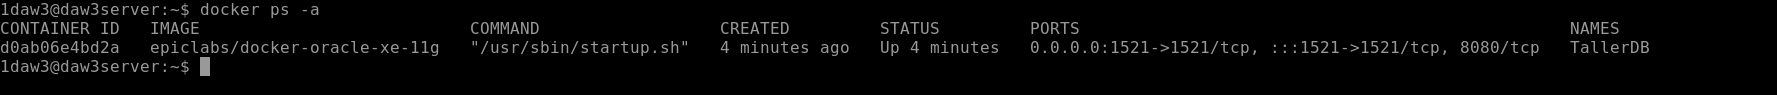
\includegraphics[width=1.0\textwidth]{CapturasSistemas/oracleEnMarcha.PNG}
    \caption{Comprobación de que el SGDB está en marcha.}
  \end{figure}
  \paragraph{Instalación Página/Servidor Web}
  En nuestro caso, hemos creado una aplicacion java (.jar) que contiene un servidor web Apache Tomcat incrustado. Esta 
  aplicación sirve el contenido HTML y CSS a traves del puerto 80. Hemos decidido crear un servicio de systemd para tener 
  el programa ejecutando en todo momento. Para ello hemos ejecutado los siguientes comandos: 
  \begin{lstlisting}
    sudo systemctl set-timezone Europe/Madrid
  \end{lstlisting}
  Con este comando hemos establecido el uso horario del servidor.
  Luego hemos creado el fichero \path{/etc/systemd/system/paginaWeb.service} con el siguiente contenido: 
  \begin{lstlisting}
    [Unit]
    Description=PaginaWebTaller
    After=syslog.target

    [Service]
    User=root
    ExecStart=/usr/bin/java -jar /home/1daw3/WebTaller-0.0.1-SNAPSHOT.jar

    [Install]
    WantedBy=multi-user.target  
  \end{lstlisting}
  Finalmente para activar este servicio hemos ejecutado los siguientes comandos:
  \begin{lstlisting}
    sudo systemctl daemon-reload
    sudo systemctl enable paginaWeb.service
    sudo systemctl start paginaWeb.service
  \end{lstlisting}
}
\subsection{FOL: Riesgos Laborales}
\subsection{Inglés}
\subsection{Consideraciones}
\subsection{Bibliografía}
\appendix
\begin{appendices}
  \section{BBDD}\label{appendix:BBDD}
  \lstset{%
  	backgroundcolor=\color{white},
      inputencoding=utf8,
    escapeinside={\%*}{*)},
    literate={á}{{\'a}}1 {é}{{\'e}}1 {í}{{\'i}}1 {ó}{{\'o}}1 {ú}{{\'u}}1 {Á}{{\'A}}1 {É}{{\'E}}1 {Í}{{\'I}}1 {Ó}{{\'O}}1 {Ú}{{\'U}}1 {ñ}{{\~n}}1 {Ñ}{{\~N}}1,
  	basicstyle=\footnotesize,
  	breakatwhitespace=false,
  	breaklines=true,
  	captionpos=b,
  	commentstyle=\color{dkgreen},
  	deletekeywords={...},
  	escapeinside={\%*}{*)},
  	extendedchars=true,
  	frame=single,
  	keepspaces=true,
  	keywordstyle=\color{blue},
  	language=SQL,
  	morekeywords={*,modify,MODIFY,...},
  	numbers=left,
  	numbersep=15pt,
  	numberstyle=\tiny,
  	rulecolor=\color{ltgray},
  	showspaces=false,
  	showstringspaces=false, 
  	showtabs=false,
  	stepnumber=1,
  	tabsize=3,
}
\begin{lstlisting}[caption=Script .sql para crear la BD (BBDD)]
    /*Creamos tablespaces*/
create tablespace administracion datafile 'administracion.dbf' size 1M autoextend on;
create tablespace taller datafile 'taller.dbf' size 1M autoextend on;

/*Creamos los usuarios*/
create user Jefe identified by "jefe_1daw3_chuleta";
alter user Jefe default tablespace administracion;
create user mech1 identified by "mech1";
alter user mech1 default tablespace taller;
create user mech2 identified by "mech2";
alter user mech2 default tablespace taller;
create user mech3 identified by "mech3";
alter user mech3 default tablespace taller;
create user mech4 identified by "mech4";
alter user mech4 default tablespace taller;
create user mech5 identified by "mech5";
alter user mech5 default tablespace taller;
create user websiteVisit identified by "webVisitor";


/*Modificamos los perfiles por defecto para que no pidan cambiar password*/
alter profile default limit PASSWORD_REUSE_TIME UNLIMITED;
alter profile DEFAULT LIMIT PASSWORD_LIFE_TIME UNLIMITED;

/*Modificamos perfil de los mecanicos, maximo 1 sesion por usuario*/
create profile sesiones_mecanico LIMIT
sessions_per_user 1
failed_login_attempts UNLIMITED;
alter user mech1 PROFILE sesiones_mecanico;
alter user mech2 PROFILE sesiones_mecanico;
alter user mech3 PROFILE sesiones_mecanico;
alter user mech4 PROFILE sesiones_mecanico;
alter user mech5 PROFILE sesiones_mecanico;

/*Modificamos perfil de visitante web*/
create profile sesiones_web LIMIT
sessions_per_user UNLIMITED;
alter user websiteVisit PROFILE sesiones_web;


/*Cremos las tablas, triggers y costraints*/
create table CLIENTE(
    ID_CLIENTE NUMBER(10) PRIMARY KEY,
    NOMBRE VARCHAR2(20) NOT NULL,
    APELLIDO VARCHAR2(30) NOT NULL,
    TELEFONO VARCHAR2(9) NOT NULL,
    DIRECCION VARCHAR2(40),
    DNI VARCHAR2(9) UNIQUE,
    CORREO VARCHAR2(20) UNIQUE
) tablespace taller;
create public synonym CLIENTE for system.CLIENTE;
CREATE SEQUENCE CLIENTES_SEQ START WITH 1;

CREATE OR REPLACE TRIGGER CLIENTES_IDS BEFORE INSERT ON CLIENTE FOR EACH ROW
BEGIN SELECT CLIENTES_SEQ.NEXTVAL INTO :NEW.ID_CLIENTE FROM DUAL;
END;
/


create table VEHICULO(
    ID_VEHICULO NUMBER(10) PRIMARY KEY,
    MODELO VARCHAR2(20),
    COLOR VARCHAR2(10),
    AÑO DATE,
    MATRICULA VARCHAR2(7) UNIQUE,
    ID_CLIENTE NUMBER(10)
) tablespace taller;
create public synonym VEHICULO for system.VEHICULO;
CREATE SEQUENCE VEHICULOS_SEQ START WITH 1;

CREATE OR REPLACE TRIGGER VEHICULOS_IDS BEFORE INSERT ON VEHICULO FOR EACH ROW
BEGIN SELECT VEHICULOS_SEQ.NEXTVAL INTO :NEW.ID_VEHICULO FROM DUAL;
END;
/


create table FACTURA(
    ID_FACTURA NUMBER(10) PRIMARY KEY,
    FECHA_ENTRADA DATE,
    PRECIO_TOTAL NUMBER(5,2),
    FECHA_FIN DATE,
    PAGADO NUMBER(1,0),
    ID_VEHICULO NUMBER(10)
) tablespace taller;
create public synonym FACTURA for system.FACTURA;
CREATE SEQUENCE FACTURA_SEQ START WITH 1;
CREATE OR REPLACE TRIGGER FACTURAS_IDS BEFORE INSERT ON FACTURA FOR EACH ROW
BEGIN SELECT FACTURA_SEQ.NEXTVAL INTO :NEW.ID_FACTURA FROM DUAL;
END;
/

create table REPARACION(
    ID_REPARACION NUMBER(10) PRIMARY KEY,
    TIEMPO_HORA DATE,
    HORAS_DURACION NUMBER(4,2),
    COMENTARIOS VARCHAR2(300),
    ID_FACTURA NUMBER(10)

) tablespace taller;
create public synonym REPARACION for system.reparacion;
CREATE SEQUENCE REPARACION_SEQ START WITH 1;
CREATE OR REPLACE TRIGGER REPARACION_IDS BEFORE INSERT ON REPARACION FOR EACH ROW
BEGIN SELECT REPARACION_SEQ.NEXTVAL INTO :NEW.ID_REPARACION FROM DUAL;
END;
/

create table piezas(
    ID_PIEZA NUMBER(10) PRIMARY KEY,
    MARCA VARCHAR2(20),
    MODELO VARCHAR2(50),
    PRECIO NUMBER(5,2),
    STOCK NUMBER(3),
    DESCRIPCION VARCHAR2(255),
    URL VARCHAR2(255),
    ID_CATEGORIA NUMBER(10)
) tablespace taller;
create public synonym PIEZAS for system.piezas;
CREATE SEQUENCE PIEZAS_SEQ START WITH 1;
CREATE OR REPLACE TRIGGER PIEZAS_IDS BEFORE INSERT ON PIEZAS FOR EACH ROW
BEGIN SELECT PIEZAS_SEQ.NEXTVAL INTO :NEW.ID_PIEZA FROM DUAL;
END;
/

create table categorias(
    ID_CATEGORIA NUMBER(10) PRIMARY KEY,
    NOMBRE VARCHAR2(40) UNIQUE
) tablespace taller;
create public synonym CATEGORIAS for system.CATEGORIAS;
CREATE SEQUENCE CATEGORIAS_SEQ START WITH 1;
CREATE OR REPLACE TRIGGER CATEGORIAS_IDS BEFORE INSERT ON CATEGORIAS FOR EACH ROW
BEGIN SELECT CATEGORIAS_SEQ.NEXTVAL INTO :NEW.ID_CATEGORIA FROM DUAL;
END;
/

create table usa(
    ID_PIEZA NUMBER(10),
    ID_REPARACION NUMBER(10),
    CANTIDAD NUMBER(3)
) tablespace taller;
create public synonym USA for system.USA;

create table Realiza(
    ID_REPARACION NUMBER(10),
    ID_EMPLEADO NUMBER(10)

) tablespace taller;
create public synonym REALIZA for system.Realiza;

create table empleado(
    ID_EMPLEADO NUMBER(10) PRIMARY KEY,
    NOMBRE VARCHAR2(10),
    APELLIDO VARCHAR2(30),
    TELEFONO VARCHAR2(9),
    DNI VARCHAR2(9) UNIQUE,
    ID_JEFE NUMBER(10)
)tablespace administracion;
create public synonym EMPLEADO for system.empleado;
CREATE SEQUENCE EMPLEADO_SEQ START WITH 1;
CREATE OR REPLACE TRIGGER EMPLEADOS_IDS BEFORE INSERT ON EMPLEADO FOR EACH ROW
BEGIN SELECT EMPLEADO_SEQ.NEXTVAL INTO :NEW.ID_EMPLEADO FROM DUAL;
END;
/

ALTER TABLE VEHICULO ADD CONSTRAINT VEHICULO_FK FOREIGN KEY (ID_CLIENTE) REFERENCES CLIENTE(ID_CLIENTE);
ALTER TABLE FACTURA ADD CONSTRAINT FACTURA_FK FOREIGN KEY (ID_VEHICULO) REFERENCES VEHICULO(ID_VEHICULO);
ALTER TABLE REPARACION ADD CONSTRAINT REP_FK FOREIGN KEY (ID_FACTURA) REFERENCES FACTURA(ID_FACTURA);
ALTER TABLE EMPLEADO ADD CONSTRAINT EMP_FK FOREIGN KEY (ID_JEFE) REFERENCES EMPLEADO(ID_EMPLEADO);
ALTER TABLE PIEZAS ADD CONSTRAINT PIEZAS_FK FOREIGN KEY (ID_CATEGORIA) REFERENCES CATEGORIAS(ID_CATEGORIA);
ALTER TABLE PIEZAS ADD CONSTRAINT COMBO_UNIC UNIQUE (MARCA,MODELO);
ALTER TABLE USA ADD CONSTRAINT USA_PK PRIMARY KEY (ID_PIEZA,ID_REPARACION);
ALTER TABLE USA ADD CONSTRAINT USA_FK1 FOREIGN KEY (ID_PIEZA) REFERENCES PIEZAS(ID_PIEZA);
ALTER TABLE USA ADD CONSTRAINT USA_FK2 FOREIGN KEY (ID_REPARACION) REFERENCES REPARACION(ID_REPARACION);
ALTER TABLE REALIZA ADD CONSTRAINT REALIZA_PK PRIMARY KEY (ID_EMPLEADO,ID_REPARACION);
ALTER TABLE REALIZA ADD CONSTRAINT REALIZA_FK1 FOREIGN KEY (ID_EMPLEADO) REFERENCES EMPLEADO(ID_EMPLEADO);
ALTER TABLE REALIZA ADD CONSTRAINT REALIZA_FK2 FOREIGN KEY (ID_REPARACION) REFERENCES REPARACION(ID_REPARACION);


ALTER TABLE CLIENTE ADD CONSTRAINT DNI_FORM CHECK (REGEXP_LIKE(DNI,'\d{8}[A-Z]$'));
ALTER TABLE CLIENTE ADD CONSTRAINT TEL_FORM CHECK (REGEXP_LIKE(TELEFONO,'\d{9}'));
ALTER TABLE CLIENTE ADD CONSTRAINT CORREO_FORM CHECK (REGEXP_LIKE(CORREO,'[A-Za-zá-ú0-9_.]*@[A-Za-zá-ú0-9_]*.[A-Za-z]*$'));
ALTER TABLE EMPLEADO ADD CONSTRAINT EMP_DNI_FORM CHECK (REGEXP_LIKE(DNI,'\d{8}[A-Z]$'));
ALTER TABLE EMPLEADO ADD CONSTRAINT EMP_TEL_FORM CHECK (REGEXP_LIKE(TELEFONO,'\d{9}'));
/*ALTER TABLE VEHICULO ADD CONSTRAINT MATR_FORM CHECK (REGEXP_LIKE(MATRICULA, ''))
*/


/*Creamos roles para usuario de administracion y mecanico, y los asignamos*/
create role rol_administrador;
grant all privileges to rol_administrador;
create role rol_mecanico;
grant create SESSION to rol_mecanico;
grant update (Stock) on Piezas to rol_mecanico;
grant insert on Piezas to rol_mecanico;
grant select on Piezas to rol_mecanico;
grant all on CLIENTE to rol_mecanico;
revoke delete on CLIENTE from rol_mecanico;
grant all on Vehiculo to rol_mecanico;
revoke delete on Vehiculo from rol_mecanico;
grant all on Factura to rol_mecanico;
revoke delete on Factura from rol_mecanico;
grant all on Reparacion to rol_mecanico;
grant all on Usa to rol_mecanico;
revoke delete on Usa from rol_mecanico;
grant all on categorias to rol_mecanico;
revoke delete on categorias from rol_mecanico;
grant insert on Realiza to rol_mecanico;
grant select on EMPLEADO to rol_mecanico;

grant select on piezas to websiteVisit;
grant select on categorias to websiteVisit;

grant rol_administrador to Jefe;
grant rol_mecanico to mech1;
grant rol_mecanico to mech2;
grant rol_mecanico to mech3;
grant rol_mecanico to mech4;
grant rol_mecanico to mech5;
alter user mech1 DEFAULT role rol_mecanico;
alter user mech2 DEFAULT role rol_mecanico;
alter user mech3 DEFAULT role rol_mecanico;
alter user mech4 DEFAULT role rol_mecanico;
alter user mech5 DEFAULT role rol_mecanico;



/*Inserts*/

/*Categorias*/
INSERT INTO CATEGORIAS(NOMBRE)VALUES('Filtros y Aceite');
INSERT INTO CATEGORIAS(NOMBRE)VALUES('Frenado');
INSERT INTO CATEGORIAS(NOMBRE)VALUES('Embrague y caja de cambios');
INSERT INTO CATEGORIAS(NOMBRE)VALUES('Óptica Faros Bombillas');
INSERT INTO CATEGORIAS(NOMBRE)VALUES('Arranque y carga');
INSERT INTO CATEGORIAS(NOMBRE)VALUES('Accesorios y Equipamiento');
INSERT INTO CATEGORIAS(NOMBRE)VALUES('Piezas Motor');



INSERT INTO PIEZAS(MARCA,MODELO,PRECIO,STOCK,DESCRIPCION,URL,ID_CATEGORIA)VALUES(
'SHELL','Helix HX8 5W40 SN 3* 5L A518', 25.50 , 10, 'Aceite de motor (aceite motor)','https://oscaro.media/catalog/images/oscjpg/zoom/1010/5l_helix_hx8_syn_5w_40_high.jpg',1);
INSERT INTO PIEZAS(MARCA,MODELO,PRECIO,STOCK,DESCRIPCION,URL,ID_CATEGORIA)VALUES(
'PETRONAS','SYNTIUM 5000 XS 5W-30 SN 4X5L', 28.90 , 21, 'Aceite de motor (aceite motor)','https://oscaro.media/catalog/images/osc360/11868700/Lv2/img19.jpg',1);
INSERT INTO PIEZAS(MARCA,MODELO,PRECIO,STOCK,DESCRIPCION,URL,ID_CATEGORIA)VALUES(
'MOBIL','Super 2000 10W40 5+1L', 34.60 , 14, 'Aceite de motor (aceite motor)','https://oscaro.media/catalog/images/oscjpg/zoom/1013/151476-51.jpg',1);
INSERT INTO PIEZAS(MARCA,MODELO,PRECIO,STOCK,DESCRIPCION,URL,ID_CATEGORIA)VALUES(
'OSCARO','5W40', 21.70 , 10, 'Aceite de motor (aceite motor)','https://oscaro.media/catalog/images/osc360/12551004/Lv2/img23.jpg',1);
INSERT INTO PIEZAS(MARCA,MODELO,PRECIO,STOCK,DESCRIPCION,URL,ID_CATEGORIA)VALUES(
'CASTROL','CASTROL Magnatec 10W-40', 29.70 , 120, 'Aceite de motor (aceite motor)','https://oscaro.media/catalog/images/oscjpg/zoom/1012/15ca1f.jpg',1);
INSERT INTO PIEZAS(MARCA,MODELO,PRECIO,STOCK,DESCRIPCION,URL,ID_CATEGORIA)VALUES(
'TOTALENERGIES','QUARTZ 9000 5W40', 33.90 , 40, 'Aceite de motor (aceite motor)','https://oscaro.media/catalog/images/oscjpg/zoom/1029/213678.jpg',1);
INSERT INTO PIEZAS(MARCA,MODELO,PRECIO,STOCK,DESCRIPCION,URL,ID_CATEGORIA)VALUES(
'ELF','EVOLUTION 900 5W40', 32.60 , 52, 'Aceite de motor (aceite motor)','https://oscaro.media/catalog/images/osc360/12549869/Lv2/img23.jpg',1);
INSERT INTO PIEZAS(MARCA,MODELO,PRECIO,STOCK,DESCRIPCION,URL,ID_CATEGORIA)VALUES(
'MOBIL','Super 2000 Formula P 10W40', 31.90 , 50, 'Aceite de motor (aceite motor)','https://oscaro.media/catalog/images/osc360/4625490/Lv2/img23.jpg',1);
INSERT INTO PIEZAS(MARCA,MODELO,PRECIO,STOCK,DESCRIPCION,URL,ID_CATEGORIA)VALUES(
'PETRONAS','SYNTIUM 7000 XS 5W30', 10.90 , 30, 'Aceite de motor (aceite motor)','https://oscaro.media/catalog/images/osc360/11868675/Lv2/img05.jpg',1);
INSERT INTO PIEZAS(MARCA,MODELO,PRECIO,STOCK,DESCRIPCION,URL,ID_CATEGORIA)VALUES(
'PETRONAS','SYNTIUM 5000 XS 5W30', 34.90 , 40, 'Aceite de motor (aceite motor)','https://oscaro.media/catalog/images/osc360/11868700/Lv2/img23.jpg',1);
    

insert into PIEZAS(MARCA,MODELO,PRECIO,STOCK,DESCRIPCION,URL,ID_CATEGORIA)VALUES ('BOSCH','0 986 494 204',44.80,4,'Juego de 4 pastillas de freno (zapata)','https://oscaro.media/catalog/images/jpg/zoom/30/0986494204phrewhco0000.jpg',2);
insert into PIEZAS(MARCA,MODELO,PRECIO,STOCK,DESCRIPCION,URL,ID_CATEGORIA)VALUES ('BREMBO','08.2536.10',85.80,4,'Discos de freno','https://oscaro.media/catalog/images/jpg/zoom/65/08253610.jpg',2);
insert into PIEZAS(MARCA,MODELO,PRECIO,STOCK,DESCRIPCION,URL,ID_CATEGORIA)VALUES ('BUDWEG CALIPER A/S','343520',121.50,3,'Pinza de freno, reacondicionada.','https://oscaro.media/catalog/images/oscjpg/zoom/114/343520.jpg',2);
insert into PIEZAS(MARCA,MODELO,PRECIO,STOCK,DESCRIPCION,URL,ID_CATEGORIA)VALUES ('BOSCH','0 986 134 428',164.90,5,'Pinza de freno','https://oscaro.media/catalog/images/jpg/zoom/30/0986134428phfrwhco0000.jpg',2);
insert into PIEZAS(MARCA,MODELO,PRECIO,STOCK,DESCRIPCION,URL,ID_CATEGORIA)VALUES ('METZGER','6250252',75.80,2,'Pinza de freno','https://oscaro.media/catalog/images/bmp/zoom/94/6250252.jpg',2);
insert into PIEZAS(MARCA,MODELO,PRECIO,STOCK,DESCRIPCION,URL,ID_CATEGORIA)VALUES ('FEBI BILSTEIN','102296',35.40,1,'Sensor, revoluciones de la rueda','https://oscaro.media/catalog/images/jpg/zoom/101/102296_1.jpg',2);
insert into PIEZAS(MARCA,MODELO,PRECIO,STOCK,DESCRIPCION,URL,ID_CATEGORIA)VALUES ('AJUSA','01107400',5.9,4,'Junta (retén)','https://oscaro.media/catalog/images/oscjpg/zoom/139/01107400.jpg',2);
insert into PIEZAS(MARCA,MODELO,PRECIO,STOCK,DESCRIPCION,URL,ID_CATEGORIA)VALUES ('ELRING','646.830',24.10,4,'Junta, bomba de vacío','https://oscaro.media/catalog/images/oscjpg/zoom/10/758044.jpg',2);
insert into PIEZAS(MARCA,MODELO,PRECIO,STOCK,DESCRIPCION,URL,ID_CATEGORIA)VALUES ('BREMBO','09.8304.21',64.60,4,'Discos de freno','https://oscaro.media/catalog/images/jpg/zoom/65/09830421.jpg',2);

insert into PIEZAS(MARCA,MODELO,PRECIO,STOCK,DESCRIPCION,URL,ID_CATEGORIA)VALUES ('LUK','602 0008 00',981.50,1,'Kit de embrague','https://oscaro.media/catalog/images/jpg/zoom/6/602000800.jpg',3);
insert into PIEZAS(MARCA,MODELO,PRECIO,STOCK,DESCRIPCION,URL,ID_CATEGORIA)VALUES ('VALEO','828060',349.90,4,'Kit de embrague','https://oscaro.media/catalog/images/jpg/zoom/21/valeo_kit3p_rb.jpg',3);
insert into PIEZAS(MARCA,MODELO,PRECIO,STOCK,DESCRIPCION,URL,ID_CATEGORIA)VALUES ('LUK','624 3474 09',230.90,2,'Kit de embrague','https://oscaro.media/catalog/images/jpg/zoom/6/09_luk_pc_single_parts_clutch.jpg',3);
insert into PIEZAS(MARCA,MODELO,PRECIO,STOCK,DESCRIPCION,URL,ID_CATEGORIA)VALUES ('VALEO','821362',136.90,4,'Kit de embrague','https://oscaro.media/catalog/images/jpg/zoom/21/821362c.jpg',3);
insert into PIEZAS(MARCA,MODELO,PRECIO,STOCK,DESCRIPCION,URL,ID_CATEGORIA)VALUES ('BLUE PRINT','ADA103012',246.90,3,'Kit de embrague','https://oscaro.media/catalog/images/jpg/zoom/350/ada103012_2.jpg',3);
insert into PIEZAS(MARCA,MODELO,PRECIO,STOCK,DESCRIPCION,URL,ID_CATEGORIA)VALUES ('AISIN','ATF-91005',51.40,3,'Aceite caja de cambios','https://oscaro.media/catalog/images/jpg/zoom/166/atf-91005%2001.jpg',3);
insert into PIEZAS(MARCA,MODELO,PRECIO,STOCK,DESCRIPCION,URL,ID_CATEGORIA)VALUES ('AISIN','CVTF-90005',53.90,2,'Aceite caja de cambios','https://oscaro.media/catalog/images/jpg/zoom/166/cvtf-90005%2001.jpg',3);
insert into PIEZAS(MARCA,MODELO,PRECIO,STOCK,DESCRIPCION,URL,ID_CATEGORIA)VALUES ('SHELL','Spirax S4G75W80',9.60,1,'Aceite caja de cambios','https://oscaro.media/catalog/images/oscjpg/zoom/1010/spirax_s4_g_75w-80%20(1).jpg',3);
insert into PIEZAS(MARCA,MODELO,PRECIO,STOCK,DESCRIPCION,URL,ID_CATEGORIA)VALUES ('CORTECO','20034710B',13.70,12,'Casquilo guía, embrague','https://oscaro.media/catalog/images/bmp/zoom/140/20034710.jpg',3);
insert into PIEZAS(MARCA,MODELO,PRECIO,STOCK,DESCRIPCION,URL,ID_CATEGORIA)VALUES ('FEBI BILSTEIN','46008',20.90,4,'Casquilo guía, embrague','https://oscaro.media/catalog/images/jpg/zoom/101/46008_1.jpg',3);


insert into PIEZAS(MARCA,MODELO,PRECIO,STOCK,DESCRIPCION,URL,ID_CATEGORIA)VALUES ('VALEO','046871',728.50,1,'Faro principal (faro delantero)','https://oscaro.media/catalog/images/jpg/zoom/21/valeo_headlamp_046871_01.jpg',4);
insert into PIEZAS(MARCA,MODELO,PRECIO,STOCK,DESCRIPCION,URL,ID_CATEGORIA)VALUES ('VAN WEZEL','2730961',34.80,4,'Faro principal (faro delantero)','https://oscaro.media/catalog/images/bmp/zoom/36/k2730961.jpg',4);
insert into PIEZAS(MARCA,MODELO,PRECIO,STOCK,DESCRIPCION,URL,ID_CATEGORIA)VALUES ('MAGNETI MARELLI','711307024171',532.90,2,'Faro principal (faro delantero)','https://oscaro.media/catalog/images/jpg/zoom/95/ilf_lpo101_wr.jpg',4);
insert into PIEZAS(MARCA,MODELO,PRECIO,STOCK,DESCRIPCION,URL,ID_CATEGORIA)VALUES ('VALEO','045437',149.90,2,'Faro principal (faro delantero)','https://oscaro.media/catalog/images/jpg/zoom/21/valeo_headlamp_045437_01.jpg',4);
insert into PIEZAS(MARCA,MODELO,PRECIO,STOCK,DESCRIPCION,URL,ID_CATEGORIA)VALUES ('VAN WEZEL','5216962',70.20,4,'Faro principal (faro delantero)','https://oscaro.media/catalog/images/bmp/zoom/36/k5216961.jpg',4);
insert into PIEZAS(MARCA,MODELO,PRECIO,STOCK,DESCRIPCION,URL,ID_CATEGORIA)VALUES ('HERTH+BUSS ELPARTS','89901311',17.40,2,'Lámpara incandescente, luz trasera (bombilla) x10','https://oscaro.media/catalog/images/jpg/normal/72/89901311.jpg',4);
insert into PIEZAS(MARCA,MODELO,PRECIO,STOCK,DESCRIPCION,URL,ID_CATEGORIA)VALUES ('PHILIPS','69741430',11.10,4,'Lámpara (bombilla). 2 x WY21 W VISION','https://oscaro.media/catalog/images/oscjpg/zoom/75/philips_pack_pr_wy21w_69741430_12071b2_s_emea_16.jpg',4);
insert into PIEZAS(MARCA,MODELO,PRECIO,STOCK,DESCRIPCION,URL,ID_CATEGORIA)VALUES ('HELLA','8GH 008 417-001',6.60,15,'Lámpara (bombilla) x 10','https://oscaro.media/catalog/images/jpg/zoom/2/k1948.jpg',4);
insert into PIEZAS(MARCA,MODELO,PRECIO,STOCK,DESCRIPCION,URL,ID_CATEGORIA)VALUES ('OSRAM','64132ULT-02B',11.60,10,'Lámpara (bombilla) 2 x H6W ULTRA LIFE','https://oscaro.media/catalog/images/jpg/zoom/67/617121-p.jpg',4);
insert into PIEZAS(MARCA,MODELO,PRECIO,STOCK,DESCRIPCION,URL,ID_CATEGORIA)VALUES ('PHILIPS','5547730',2.10,1,'Lámpara (bombilla) 2 x R10W VISION','https://oscaro.media/catalog/images/oscjpg/zoom/75/philips_pack_pr_r10w_05547730_12814b2_s_emea_16.jpg',4);

insert into PIEZAS(MARCA,MODELO,PRECIO,STOCK,DESCRIPCION,URL,ID_CATEGORIA)VALUES ('TUDOR','TB450',89.90,1,'Batería 45 Ah','https://oscaro.media/catalog/images/jpg/zoom/212/tb450new%20copie.jpg',5);
insert into PIEZAS(MARCA,MODELO,PRECIO,STOCK,DESCRIPCION,URL,ID_CATEGORIA)VALUES ('NIPPON','U540L17B',76.80,10,'Batería 50 Ah','https://oscaro.media/catalog/images/jpg/zoom/440/u540l17ba.jpg',5);
insert into PIEZAS(MARCA,MODELO,PRECIO,STOCK,DESCRIPCION,URL,ID_CATEGORIA)VALUES ('YUASA','YBX5335',89.90,1,'Batería 100 Ah','https://oscaro.media/catalog/images/oscjpg/zoom/4451/yuasaybx5335.jpg',5);
insert into PIEZAS(MARCA,MODELO,PRECIO,STOCK,DESCRIPCION,URL,ID_CATEGORIA)VALUES ('NIPPON','U540L05B',64.90,0,'Batería 35 Ah','https://oscaro.media/catalog/images/jpg/zoom/440/u540l05ba.jpg',5);
insert into PIEZAS(MARCA,MODELO,PRECIO,STOCK,DESCRIPCION,URL,ID_CATEGORIA)VALUES ('VARTA','5401260333132',66.90,4,'Batería 40 Ah','https://oscaro.media/catalog/images/jpg/zoom/26/540126033_jpg.jpg',5);
insert into PIEZAS(MARCA,MODELO,PRECIO,STOCK,DESCRIPCION,URL,ID_CATEGORIA)VALUES ('YUASA','YBX5334',96.90,2,'Batería 100 Ah','https://oscaro.media/catalog/images/jpg/zoom/4451/img_929_4871367.jpg',5);
insert into PIEZAS(MARCA,MODELO,PRECIO,STOCK,DESCRIPCION,URL,ID_CATEGORIA)VALUES ('YUASA','YBX3054',52.60,1,'Batería 36 Ah','https://oscaro.media/catalog/images/jpg/zoom/4451/img_954_4131630.jpg',5);
insert into PIEZAS(MARCA,MODELO,PRECIO,STOCK,DESCRIPCION,URL,ID_CATEGORIA)VALUES ('BOSCH','0 092 S4E 420',147.90,2,'Batería 85 Ah','https://oscaro.media/catalog/images/jpg/zoom/30/0092s4e420dranwhco00mm.jpg',5);
insert into PIEZAS(MARCA,MODELO,PRECIO,STOCK,DESCRIPCION,URL,ID_CATEGORIA)VALUES ('BOSCH','0 092 S4E 400',125.50,1,'Batería 65 Ah','https://oscaro.media/catalog/images/jpg/zoom/30/0092s4e400dranwhgr00mm.jpg',5);
insert into PIEZAS(MARCA,MODELO,PRECIO,STOCK,DESCRIPCION,URL,ID_CATEGORIA)VALUES ('VARTA','5954040833132',153.50,1,'Batería 95 Ah','https://oscaro.media/catalog/images/oscjpg/zoom/26/595404083.jpg',5);

insert into PIEZAS(MARCA,MODELO,PRECIO,STOCK,DESCRIPCION,URL,ID_CATEGORIA)VALUES ('DBS','01763194',59.90,2,'Alfombrilla a medida','https://oscaro.media/catalog/images/oscjpg/zoom/1052/tapis_star_1.jpg',6);
insert into PIEZAS(MARCA,MODELO,PRECIO,STOCK,DESCRIPCION,URL,ID_CATEGORIA)VALUES ('DBS','01765706',49.90,2,'Alfombrilla a medida','https://oscaro.media/catalog/images/oscjpg/zoom/1052/star1.jpg',6);
insert into PIEZAS(MARCA,MODELO,PRECIO,STOCK,DESCRIPCION,URL,ID_CATEGORIA)VALUES ('DBS','01766017',42.40,1,'Alfombrilla a medida','https://oscaro.media/catalog/images/oscjpg/zoom/1052/3261887670176.jpg',6);
insert into PIEZAS(MARCA,MODELO,PRECIO,STOCK,DESCRIPCION,URL,ID_CATEGORIA)VALUES ('DBS','01764109',34.90,4,'Alfombrilla a medida','https://oscaro.media/catalog/images/oscjpg/zoom/1052/tapis_luxe_1.jpg',6);
insert into PIEZAS(MARCA,MODELO,PRECIO,STOCK,DESCRIPCION,URL,ID_CATEGORIA)VALUES ('DBS','01765700',24.40,1,'Alfombrilla a medida','https://oscaro.media/catalog/images/oscjpg/zoom/1052/star1.jpg',6);
insert into PIEZAS(MARCA,MODELO,PRECIO,STOCK,DESCRIPCION,URL,ID_CATEGORIA)VALUES ('VALEO','632001',158.90,1,'Sensor de marcha atrás (sensor de aparcamiento)','https://oscaro.media/catalog/images/oscjpg/zoom/21/632001.jpg',6);
insert into PIEZAS(MARCA,MODELO,PRECIO,STOCK,DESCRIPCION,URL,ID_CATEGORIA)VALUES ('BEEPER','REM101',34.90,0,'Sensor de marcha atrás (sensor de aparcamiento)','https://oscaro.media/catalog/images/oscjpg/zoom/1042/rem101%201%20photo%20principale.jpg',6);
insert into PIEZAS(MARCA,MODELO,PRECIO,STOCK,DESCRIPCION,URL,ID_CATEGORIA)VALUES ('BEEPER','RE002A/4-B',42.20,0,'Sensor de marcha atrás (sensor de aparcamiento)','https://oscaro.media/catalog/images/oscjpg/zoom/1042/radar-de-recul-re002a-4-b_1.jpg',6);
insert into PIEZAS(MARCA,MODELO,PRECIO,STOCK,DESCRIPCION,URL,ID_CATEGORIA)VALUES ('VALEO','632202',212.90,2,'Sensor de marcha atrás (sensor de aparcamiento)','https://oscaro.media/catalog/images/jpg/zoom/21/assembly_kit_632202_01.jpg',6);
insert into PIEZAS(MARCA,MODELO,PRECIO,STOCK,DESCRIPCION,URL,ID_CATEGORIA)VALUES ('VALEO','632201',141.90,1,'Sensor de marcha atrás (sensor de aparcamiento)','https://oscaro.media/catalog/images/jpg/zoom/21/assembly_kit_632201_01.jpg',6);

insert into PIEZAS(MARCA,MODELO,PRECIO,STOCK,DESCRIPCION,URL,ID_CATEGORIA)VALUES ('BOSCH','0 445 110 102',239.50,23,'Inyector','https://oscaro.media/catalog/images/osc360/69324/Lv2/img23.jpg',7);
insert into PIEZAS(MARCA,MODELO,PRECIO,STOCK,DESCRIPCION,URL,ID_CATEGORIA)VALUES ('SKF','VKMA 33165',46.40,15,'Juego de correas auxiliares servicios','https://oscaro.media/catalog/images/bmp/zoom/50/vkma%2033165.jpg',7);
insert into PIEZAS(MARCA,MODELO,PRECIO,STOCK,DESCRIPCION,URL,ID_CATEGORIA)VALUES ('RCA FRANCE',' RCA7086392X',296.50,3,'Turbocompresor. Este kit de turbo contiene un kit de juntas y una dosis de aceite.','https://oscaro.media/catalog/images/jpg/zoom/492/rca7086392x.jpg',7);
insert into PIEZAS(MARCA,MODELO,PRECIO,STOCK,DESCRIPCION,URL,ID_CATEGORIA)VALUES ('VALEO','506018',34.40,15,'Bomba de agua.','https://oscaro.media/catalog/images/osc360/668965/Lv2/img23.jpg',7);
insert into PIEZAS(MARCA,MODELO,PRECIO,STOCK,DESCRIPCION,URL,ID_CATEGORIA)VALUES ('MAHLE AFTERMARKET','607VE31078000',11.30,20,'Válvula de admisión','https://oscaro.media/catalog/images/osc360/2218452/Lv2/img23.jpg',7);
insert into PIEZAS(MARCA,MODELO,PRECIO,STOCK,DESCRIPCION,URL,ID_CATEGORIA)VALUES ('VAN WEZEL','1747072',86.40,1,'Cárter de aceite','https://oscaro.media/catalog/images/bmp/zoom/36/i1747072.jpg',7);
insert into PIEZAS(MARCA,MODELO,PRECIO,STOCK,DESCRIPCION,URL,ID_CATEGORIA)VALUES ('VAN WEZEL','1754074',27.90,3,'Cárter de aceite','https://oscaro.media/catalog/images/jpg/zoom/36/i1754074.jpg',7);
insert into PIEZAS(MARCA,MODELO,PRECIO,STOCK,DESCRIPCION,URL,ID_CATEGORIA)VALUES ('PAYEN','AG5210',31.60,5,'Junta, culata','https://oscaro.media/catalog/images/jpg/zoom/113/img_2811_2016080217345186609.jpg',7);
insert into PIEZAS(MARCA,MODELO,PRECIO,STOCK,DESCRIPCION,URL,ID_CATEGORIA)VALUES ('VALEO','255101',12.60,10,'Sensor, presión de aceite','https://oscaro.media/catalog/images/jpg/zoom/21/sensor_oil_pressure_255101_01.jpg',7);
insert into PIEZAS(MARCA,MODELO,PRECIO,STOCK,DESCRIPCION,URL,ID_CATEGORIA)VALUES ('BOSCH','0 986 345 007',11.70,9,'Sensor, presión de aceite','https://oscaro.media/catalog/images/bmp/zoom/30/f0986345007.jpg',7);

insert into cliente(nombre,apellido,telefono,direccion,dni) values('Miguel','Fernandez','624232910','Madrid,Calle Lorenzo 40, 2B','45199189P');
insert into cliente(nombre,apellido,telefono,direccion,dni) values('Felipe','Gonzalez','645262911','Irún,Calle Oscura 2','41293189K');
insert into cliente(nombre,apellido,telefono,direccion,dni) values('Paco','El Del Bar','642222111','Madrid,Calle Zapatazo 40','14144189A');
insert into cliente(nombre,apellido,telefono,direccion,dni) values('Jaime','Alvarez','623222111','Zaragoza,Calle Roberto 22, 1A','45122279K');
insert into cliente(nombre,apellido,telefono,direccion,dni) values('Aitor','Arconada','644112111','Madrid,Calle Lorenzo 40, 2A','46197159N');
insert into cliente(nombre,apellido,telefono,direccion,dni,correo) values ('Elena','Villazul','644622611','Hondarribia, Soroetaberri 10, 2A','46197159K','EleVil@gmail.com');
insert into cliente(nombre,apellido,telefono,direccion,dni,correo) values  ('Ane','Perez','644789111','Guijuelo, Calle Jamón 2, 5A','46195159N','AnePer@gmail.com');
insert into cliente(nombre,apellido,telefono,direccion,dni,correo) values ('Julia','Bilbao','698712111','Gijón, Calle Sidrera ,3 Derecha','46567959A','JulBil@gmail.com');
insert into cliente(nombre,apellido,telefono,direccion,dni,correo) values ('Martina','Martinis','677122111','Irún, Calle Clara 3','44195679A','MarMar@gmail.com');
insert into cliente(nombre,apellido,telefono,direccion,dni,correo) values ('Gonzala','Gonzolo','614392910','Irún, Paseo Colon 30, 2A','46197167S','GonGOn@gmail.com');


/*jefe*/

insert into empleado(NOMBRE,APELLIDO,TELEFONO,DNI)VALUES
('Juan','Rodriguez','623748765','74416412V');
/*empleados*/
insert into empleado(NOMBRE,APELLIDO,TELEFONO,DNI,ID_JEFE)VALUES
('Raul','Iruretagollena','678123451','48125689U',1);

insert into empleado(NOMBRE,APELLIDO,TELEFONO,DNI,ID_JEFE)VALUES
('Juanjo','Uriburu','712345623','56781243T',1);

insert into empleado(NOMBRE,APELLIDO,TELEFONO,DNI,ID_JEFE)VALUES
('Aitor','Segurola','678908712','71142398P',1);

insert into empleado(NOMBRE,APELLIDO,TELEFONO,DNI,ID_JEFE)VALUES
('Sonia','Virasoro','678954321','87659823M',1);

insert into empleado(NOMBRE,APELLIDO,TELEFONO,DNI,ID_JEFE)VALUES
('JuanMari','Peralta','711232455','44671231R',1);
commit;


insert into vehiculo(MODELO,COLOR,AÑO,MATRICULA,ID_CLIENTE)VALUES(
    'FIAT','BLANCO',TO_DATE('2012','yyyy'),'3465PCR',10
);
insert into vehiculo(MODELO,COLOR,AÑO,MATRICULA,ID_CLIENTE)VALUES(
    'PEUGEOT','ROJO',TO_DATE('2019','yyyy'),'7775SLP',9
);
insert into vehiculo(MODELO,COLOR,AÑO,MATRICULA,ID_CLIENTE)VALUES(
    'MERCEDES','PLATEADO',TO_DATE('2015','yyyy'),'5552BNJ',8
);
insert into vehiculo(MODELO,COLOR,AÑO,MATRICULA,ID_CLIENTE)VALUES(
    'BMW','VERDE',TO_DATE('2019','yyyy'),'5443TYV',7
);
insert into vehiculo(MODELO,COLOR,AÑO,MATRICULA,ID_CLIENTE)VALUES(
    'TOYOTA','CREMA',TO_DATE('2020','yyyy'),'6784CBS',6
);
insert into vehiculo(MODELO,COLOR,AÑO,MATRICULA,ID_CLIENTE)VALUES(
    'RENAULT','ROJO',TO_DATE('2021','yyyy'),'7886RSE',5
);
insert into vehiculo(MODELO,COLOR,AÑO,MATRICULA,ID_CLIENTE)VALUES(
    'MERCEDES','GRANATE',TO_DATE('2014','yyyy'),'7845NHT',4
);
insert into vehiculo(MODELO,COLOR,AÑO,MATRICULA,ID_CLIENTE)VALUES(
    'AUDI','NEGRO',TO_DATE('2020','yyyy'),'6784UOL',3
);
insert into vehiculo(MODELO,COLOR,AÑO,MATRICULA,ID_CLIENTE)VALUES(
    'VOLKSWAGEN','AZUL',TO_DATE('2006','yyyy'),'7894FUB',2
);
insert into vehiculo(MODELO,COLOR,AÑO,MATRICULA,ID_CLIENTE)VALUES(
    'FIAT','GRIS',TO_DATE('2016','yyyy'),'8934KOL',1
);
insert into vehiculo(MODELO,COLOR,AÑO,MATRICULA,ID_CLIENTE)VALUES(
    'BMW','AMARILLO',TO_DATE('2019','yyyy'),'8923DFT',8
);
insert into vehiculo(MODELO,COLOR,AÑO,MATRICULA,ID_CLIENTE)VALUES(
    'REANAULT','BLANCO',TO_DATE('2012','yyyy'),'7839OPL',9
);

\end{lstlisting}
  \section{Programación}\label{appendix:programacion}
  \subsection{Paquete Modelos}
  \definecolor{pblue}{rgb}{0.13,0.13,1}
\definecolor{pgreen}{rgb}{0,0.5,0}
\definecolor{pred}{rgb}{0.9,0,0}
\definecolor{pgrey}{rgb}{0.46,0.45,0.48}


\lstset{language=Java,
backgroundcolor=\color{white},
inputencoding=utf8,
escapeinside={\%*}{*)},
literate={á}{{\'a}}1 {é}{{\'e}}1 {í}{{\'i}}1 {ó}{{\'o}}1 {ú}{{\'u}}1 {Á}{{\'A}}1 {É}{{\'E}}1 {Í}{{\'I}}1 {Ó}{{\'O}}1 {Ú}{{\'U}}1 {ñ}{{\~n}}1 {Ñ}{{\~N}}1,
breakatwhitespace=false,
  showspaces=false,
  showtabs=false,
  breaklines=true,
  showstringspaces=false,
  breakatwhitespace=true,
  commentstyle=\color{pgreen},
  keywordstyle=\color{pblue},
  stringstyle=\color{pred},
  basicstyle=\ttfamily,
  moredelim=[il][\textcolor{pgrey}]{$$},
  moredelim=[is][\textcolor{pgrey}]{\%\%}{\%\%}
}
\begin{lstlisting}[caption=Categoria.java (LMSI)]
package com.Taller.WebTaller.modelos;

public class Categoria {
    public String getNombre() {
        return nombre;
    }

    public void setNombre(String nombre) {
        this.nombre = nombre;
    }

    private String nombre;
}
\end{lstlisting}
\clearpage
\begin{lstlisting}[caption=Marca.java (LMSI)]
  
package com.Taller.WebTaller.modelos;

public class Marca {

    private String marca;
    private int cantidad;

    public String getMarca() {
        return marca;
    }

    public void setMarca(String marca) {
        this.marca = marca;
    }

    public int getCantidad() {
        return cantidad;
    }

    public void setCantidad(int cantidad) {
        this.cantidad = cantidad;
    }
}
\end{lstlisting}
\clearpage
\begin{lstlisting}[caption=Pieza.java (LMSI)]
package com.Taller.WebTaller.modelos;

public class Pieza {
    private int id_pieza;
    private String marca;
    private String modelo;
    private float precio;
    private String url;
    private String descripcion;
    private int stock;
    private String categoria;

    public int getId_pieza() {
        return id_pieza;
    }

    public void setId_pieza(int id_pieza) {
        this.id_pieza = id_pieza;
    }

    public float getPrecio() {
        return precio;
    }

    public void setPrecio(float precio) {
        this.precio = precio;
    }

    public String getMarca() {
        return marca;
    }

    public void setMarca(String marca) {
        this.marca = marca;
    }

    public String getModelo() {
        return modelo;
    }

    public void setModelo(String modelo) {
        this.modelo = modelo;
    }

    public String getDescripcion() {
        return descripcion;
    }

    public void setDescripcion(String descripcion) {
        this.descripcion = descripcion;
    }

    public int getStock() {
        return stock;
    }

    public void setStock(int stock) {
        this.stock = stock;
    }

    public String getCategoria() {
        return categoria;
    }

    public void setCategoria(String categoria) {
        this.categoria = categoria;
    }

    public String getUrl() {
        return url;
    }

    public void setUrl(String url) {
        this.url = url;
    }
}
\end{lstlisting}
\clearpage
  \subsection{Paquete DAO}
  \definecolor{pblue}{rgb}{0.13,0.13,1}
\definecolor{pgreen}{rgb}{0,0.5,0}
\definecolor{pred}{rgb}{0.9,0,0}
\definecolor{pgrey}{rgb}{0.46,0.45,0.48}


\lstset{language=Java,
backgroundcolor=\color{white},
inputencoding=utf8,
escapeinside={\%*}{*)},
literate={á}{{\'a}}1 {é}{{\'e}}1 {í}{{\'i}}1 {ó}{{\'o}}1 {ú}{{\'u}}1 {Á}{{\'A}}1 {É}{{\'E}}1 {Í}{{\'I}}1 {Ó}{{\'O}}1 {Ú}{{\'U}}1 {ñ}{{\~n}}1 {Ñ}{{\~N}}1,
breakatwhitespace=false,
  showspaces=false,
  showtabs=false,
  breaklines=true,
  showstringspaces=false,
  breakatwhitespace=true,
  commentstyle=\color{pgreen},
  keywordstyle=\color{pblue},
  stringstyle=\color{pred},
  basicstyle=\ttfamily,
  moredelim=[il][\textcolor{pgrey}]{$$},
  moredelim=[is][\textcolor{pgrey}]{\%\%}{\%\%}
}
\begin{lstlisting}[caption=PiezaDao.java (LMSI)]
package com.Taller.WebTaller.dao;

import com.Taller.WebTaller.modelos.Categoria;
import com.Taller.WebTaller.modelos.Marca;
import com.Taller.WebTaller.modelos.Pieza;

import java.util.ArrayList;
import java.util.List;

public interface PiezaDao {

    public List<Pieza> LeerPiezasTodas();
    public List<Pieza> LeerPorMarca(String marca);
    public List<Pieza> LeerPorCategoria(String categoria);
    public List<Marca> ListaMarcas();
    public List<Categoria> ListaCategorias();
    public Pieza piezaPorId(int id);
}
\end{lstlisting}
\clearpage
\begin{lstlisting}[caption=PiezaDaoTodos.java (LMSI)]
package com.Taller.WebTaller.dao;


import com.Taller.WebTaller.modelos.Categoria;
import com.Taller.WebTaller.modelos.Marca;
import com.Taller.WebTaller.modelos.Pieza;
import org.springframework.stereotype.Repository;
import org.springframework.beans.factory.annotation.Autowired;
import org.springframework.jdbc.core.BeanPropertyRowMapper;
import org.springframework.jdbc.core.JdbcTemplate;

import java.util.List;

@Repository
public class PiezaDaoTodos implements PiezaDao{

    @Autowired
    private JdbcTemplate jdbcTemplate;
    @Override
    public List<Pieza> LeerPiezasTodas() {
        String sql = "SELECT id_pieza, marca, modelo, precio, descripcion, stock,url, categorias.nombre as categoria FROM piezas inner join categorias on piezas.id_categoria = categorias.id_categoria";

        return  jdbcTemplate.query(sql,
                BeanPropertyRowMapper.newInstance(Pieza.class));
    }

    @Override
    public List<Pieza> LeerPorMarca(String marca) {
        String sql = "SELECT id_pieza, marca, modelo, precio, descripcion, stock, url, categorias.nombre as categoria FROM piezas inner join categorias on piezas.id_categoria = categorias.id_categoria where marca='"+marca+"'";

        return  jdbcTemplate.query(sql,
                BeanPropertyRowMapper.newInstance(Pieza.class));
    }

    @Override
    public List<Pieza> LeerPorCategoria(String categoria) {
        String sql = "SELECT id_pieza, marca, modelo, precio, descripcion, stock, url, categorias.nombre as categoria FROM piezas inner join categorias on piezas.id_categoria = categorias.id_categoria where categorias.nombre='"+categoria+"'";
        return jdbcTemplate.query(sql,
                BeanPropertyRowMapper.newInstance(Pieza.class));
    }

    @Override
    public List<Marca> ListaMarcas(){
        String sql = "select marca, count(*) as cantidad from PIEZAS group by marca";
        return jdbcTemplate.query(sql,
                BeanPropertyRowMapper.newInstance(Marca.class));
    }
    @Override
    public List<Categoria> ListaCategorias(){
        String sql = "select nombre from categorias";
        return jdbcTemplate.query(sql,
                BeanPropertyRowMapper.newInstance(Categoria.class));
    }

    @Override
    public Pieza piezaPorId(int id) {
        String sql = "select id_pieza,marca,modelo,precio,descripcion,stock,url from piezas where id_pieza="+id;
        return  jdbcTemplate.queryForObject(sql,
                BeanPropertyRowMapper.newInstance(Pieza.class));
    }
}
\end{lstlisting}
\clearpage
  \subsection{Paquete System}
  \definecolor{pblue}{rgb}{0.13,0.13,1}
\definecolor{pgreen}{rgb}{0,0.5,0}
\definecolor{pred}{rgb}{0.9,0,0}
\definecolor{pgrey}{rgb}{0.46,0.45,0.48}


\lstset{language=Java,
backgroundcolor=\color{white},
inputencoding=utf8,
escapeinside={\%*}{*)},
literate={á}{{\'a}}1 {é}{{\'e}}1 {í}{{\'i}}1 {ó}{{\'o}}1 {ú}{{\'u}}1 {Á}{{\'A}}1 {É}{{\'E}}1 {Í}{{\'I}}1 {Ó}{{\'O}}1 {Ú}{{\'U}}1 {ñ}{{\~n}}1 {Ñ}{{\~N}}1,
basicstyle=\footnotesize,
breakatwhitespace=false,
  showspaces=false,
  showtabs=false,
  breaklines=true,
  showstringspaces=false,
  breakatwhitespace=true,
  commentstyle=\color{pgreen},
  keywordstyle=\color{pblue},
  stringstyle=\color{pred},
  basicstyle=\ttfamily,
  moredelim=[il][\textcolor{pgrey}]{$$},
  moredelim=[is][\textcolor{pgrey}]{\%\%}{\%\%}
}

\begin{lstlisting}[caption=GestorOperaciones.java (App Escritorio)]
    package System;

    import java.sql.SQLException;
    import java.util.ArrayList;
    import java.util.Date;
    import java.util.Map.Entry;
    
    import DAO.Consultas;
    import DAO.Inserts;
    import DAO.Updates;
    import Modelos.Factura;
    import Modelos.Pieza;
    import Modelos.Reparacion;
    import Modelos.Vehiculo;
    public class GestorOperaciones {
        
        private String username;
        private String password;
        private ArrayList<Vehiculo> coches;
        private ArrayList<Factura> facturas;
        private ArrayList<Pieza> piezas;
        private ArrayList<Reparacion> reparaciones; 
        private Consultas consultasDB;
        private Inserts insertsDB;
        private Updates updatesDB;
        
        public GestorOperaciones(String username, String password) throws SQLException {
            this.username=username;
            this.password=password;
            consultasDB = new Consultas(username,password);
            insertsDB = new Inserts(username,password);
            updatesDB = new Updates(username,password);
            /*Obtenemos los datos de la base de datos*/
            coches = consultasDB.verVehiculos();
            piezas = consultasDB.verPiezas();
            facturas = consultasDB.verFacturas();
            reparaciones = consultasDB.verReparaciones();
            /*Asignamos el vehiculo a cada factura usando las claves primarias*/
            facturas.forEach(factura ->{
                factura.setCoche( buscarPorID( factura.getId_vehiculo() ));
            });
            /*Asignamos a que factura corresponde cada reparacion.*/
            reparaciones.forEach(rep ->{
                Factura factura = buscarFacturaPorId(rep.getId_factura());
                factura.getReparaciones().add(rep);
            });
        }
        
        /*Devuelve la factura con el ID especificado*/
        private Factura buscarFacturaPorId(int id) {
            for(Factura factura : facturas) {
                if (factura.getId()==id) return factura;
            }
            return null;
        }
        
        /*Devuelve el vehiculo con el ID buscado*/
        private Vehiculo buscarPorID(int id) {
            for(Vehiculo coche : coches) {
                if (coche.getId()==id) return coche;
            }
            return null;
        }
        
        /*Devuelve una factura abierta del coche. Si no la encuentra le crea una nueva y la escribe en la base de datos*/
        public Factura buscarFacturaActualCoche(Vehiculo coche) throws SQLException {
            for(Factura factura : facturas) {
                if (factura.getCoche()==coche && factura.getFecha_fin()==null) {
                    return factura;
                }
            }
            
            /*En caso de que sea nueva factura, la escribimos en la base de datos y obtenemos su id*/
            Factura factura = new Factura(coche);
            insertsDB.insertarFactura(factura);
            factura.setId(consultasDB.last_factura_id());
            facturas.add(factura);
            return factura;
        }
    
        /*Actualiza el stock de la pieza restando la cantidad introducida*/
        private void restarPiezas(Pieza pieza, int cantidad) throws SQLException {
            updatesDB.restarStockPieza(pieza, cantidad);
            pieza.setStock(pieza.getStock()-cantidad);
        }
        
        public ArrayList<Pieza> piezasEnStock(){
            ArrayList<Pieza> piezerio = new ArrayList<Pieza>();
            piezas.forEach(piez -> {
                if (piez.getStock()>0) piezerio.add(piez);
            });
            return piezerio;
        }
        /*
         Guarda la reparacion en la base de datos, junto a todas la lineas correspondientes de la tabla USA (piezas-cantidad-reparacion)
         Tambien actualiza el stock de piezas de la tabla piezas.
          */
        public void anadirReparacion(Reparacion rep) throws SQLException {
            insertsDB.insertarReparacion(rep);
            for (Entry<Pieza,Integer> linea : rep.getPiezas().entrySet()) {
                restarPiezas(linea.getKey(),linea.getValue());
            }
        }
        
        /*Cuando un vehiculo ha sido totalmente reparado (1 o mas reparaciones)
         Sobre escribe la linea en la tabla factura, actualizando el precio total, la fecha fin y si esta pagado o no. 
         */
        public void terminarReparacionCoche(Factura factura) throws SQLException {
            factura.setFecha_fin(new Date());
            /*Hacer update en lugar de insert*/
            updatesDB.actualizarFactura(factura);
        }
        
        /*Añade piezas a la reparacion vigente*/
        public void anadirPiezasReparacion(Pieza pieza,int cantidad,Reparacion rep) {
            rep.getPiezas().put(pieza, cantidad);
        }
        
        public ArrayList<Vehiculo> vehiculosEnReparacion(){
            ArrayList<Vehiculo> vehiculos = new ArrayList<Vehiculo>();
            facturas.forEach(factura ->{
                if (factura.getFecha_fin()==null) vehiculos.add(factura.getCoche());
            });
            return vehiculos;
        }
    
        public ArrayList<Vehiculo> getCoches() {
            return coches;
        }
    
        public void setCoches(ArrayList<Vehiculo> coches) {
            this.coches = coches;
        }
    
        public ArrayList<Factura> getFacturas() {
            return facturas;
        }
    
        public void setFacturas(ArrayList<Factura> facturas) {
            this.facturas = facturas;
        }
    
        public ArrayList<Pieza> getPiezas() {
            return piezas;
        }
    
        public void setPiezas(ArrayList<Pieza> piezas) {
            this.piezas = piezas;
        }
    
        public ArrayList<Reparacion> getReparaciones() {
            return reparaciones;
        }
    
        public void setReparaciones(ArrayList<Reparacion> reparaciones) {
            this.reparaciones = reparaciones;
        }	
        
        
    }
    
    
\end{lstlisting}
\clearpage

\begin{lstlisting}[caption=CreadorPDF.java (App Escritorio)]
    package System;

    import java.awt.Color;
    import java.io.File;
    import java.io.FileNotFoundException;
    import java.io.FileOutputStream;
    import java.io.IOException;
    import java.net.MalformedURLException;
    import java.net.URL;
    import java.util.Map.Entry;
    
    import com.itextpdf.io.image.ImageData;
    import com.itextpdf.io.image.ImageDataFactory;
    import com.itextpdf.io.image.ImageType;
    import com.itextpdf.kernel.geom.PageSize;
    import com.itextpdf.kernel.pdf.*;
    import com.itextpdf.layout.*;
    import com.itextpdf.layout.borders.Border;
    import com.itextpdf.layout.borders.DashedBorder;
    import com.itextpdf.layout.borders.DoubleBorder;
    import com.itextpdf.layout.borders.SolidBorder;
    import com.itextpdf.layout.element.BlockElement;
    import com.itextpdf.layout.element.Div;
    import com.itextpdf.layout.element.Image;
    import com.itextpdf.layout.element.List;
    import com.itextpdf.layout.element.ListItem;
    import com.itextpdf.layout.element.Paragraph;
    import com.itextpdf.layout.element.Table;
    import com.itextpdf.layout.element.Text;
    import com.itextpdf.layout.property.ListNumberingType;
    
    import Modelos.Pieza;
    import Modelos.Factura;
    import Modelos.Reparacion;
    
    
    
    
    public class CreadorPDF {
        
        
        private static final Border bordeDoble = new DoubleBorder(1.0f);
        private static final Border bordeSolido = new SolidBorder(1.0f);
        private static final Border borde_seccion = new DashedBorder(1.0f);
        
        public static void crearPdfFactura(Factura factura) throws FileNotFoundException {
            String dest = "facturas/Factura "+factura.getId()+".pdf";
            File file = new File(dest);
            file.getParentFile().mkdirs();
    
            //Inicializar escritor pdf
            FileOutputStream fos = new FileOutputStream(dest);
            PdfWriter writer = new PdfWriter(fos);
            
            //Inicializar documento pdf
            PdfDocument pdf = new PdfDocument(writer);
            
            //Inicializar documento
            Document documento = new Document(pdf,PageSize.A4);
            //Escribir en el documento
            Paragraph cabezero = new Paragraph();
    
            try {
                String url = "/Resources/imagenes/llave-inglesa.png";
                ImageData data = ImageDataFactory.create (CreadorPDF.class.getResource( "/Resources/imagenes/llave-inglesa.png" ));
                Image img = new Image(data);
                cabezero.add(img);
            } catch (Exception e1) {
                // TODO Auto-generated catch block
                e1.printStackTrace();
            }
            cabezero.add(new Text("Hermanos Gutierrez S.A").setFontSize(20f));
            documento.add(cabezero);
            documento.add( new Paragraph("Cliente : " + factura.getCoche().getDueno().toString()) .setBorder(borde_seccion));
            documento.add(new Paragraph("Vehiculo: "+ factura.getCoche().toString()) .setBorder(borde_seccion));
            documento.add(new Paragraph("Fecha entrada: "+ factura.getFecha_entrada()) .setBorder(borde_seccion));
            documento.add(new Paragraph("Fecha Fin: "+ factura.getFecha_fin()) .setBorder(borde_seccion));
            documento.add(new Paragraph("Operaciones:"));
            List lista = new List( ListNumberingType.DECIMAL ) .setBorder(bordeSolido);
            for (Reparacion rep : factura.getReparaciones()) {
                ListItem reparacion = new ListItem();
                
                reparacion.add(new Paragraph("Descripcion de operacion: "+ rep.getComentarios()));
                Table piezas = new Table(4);
                piezas.addHeaderCell("Marca");
                piezas.addHeaderCell("Modelo");
                piezas.addHeaderCell("Precio Ud");
                piezas.addHeaderCell("Cantidad");
                try {
                    for (Entry<Pieza,Integer> linea : rep.getPiezas().entrySet()) {
                        piezas.startNewRow();
                        piezas.addCell(linea.getKey().getMarca());
                        piezas.addCell(linea.getKey().getModelo());
                        piezas.addCell( Double.toString( linea.getKey().getPrecio() ));
                        piezas.addCell(Integer.toString(linea.getValue()));
                    }
                    reparacion.add(piezas);
                } catch(Exception e) {
                    //En caso de una operacion sin piezas
                }
                reparacion.add(new Paragraph("Mano de obra: "+ 10*rep.getDuracion()+"\u20ac"));
                lista.add(reparacion);
    
            } 
            documento.add(lista);
            
            documento.add(new Paragraph("Total piezas y mano de obra: "+ factura.getPrecio_total() + "\u20ac") .setBorder(bordeDoble));
            
            documento.close();
            try {
                java.awt.Desktop.getDesktop().edit(file);
            } catch (IOException e) {
                // TODO Auto-generated catch block
                e.printStackTrace();
            }
        }
    }
\end{lstlisting}
\clearpage
  \subsection{Paquete UI}
  \definecolor{pblue}{rgb}{0.13,0.13,1}
\definecolor{pgreen}{rgb}{0,0.5,0}
\definecolor{pred}{rgb}{0.9,0,0}
\definecolor{pgrey}{rgb}{0.46,0.45,0.48}


\lstset{language=Java,
backgroundcolor=\color{white},
inputencoding=utf8,
escapeinside={\%*}{*)},
literate={á}{{\'a}}1 {é}{{\'e}}1 {í}{{\'i}}1 {ó}{{\'o}}1 {ú}{{\'u}}1 {Á}{{\'A}}1 {É}{{\'E}}1 {Í}{{\'I}}1 {Ó}{{\'O}}1 {Ú}{{\'U}}1 {ñ}{{\~n}}1 {Ñ}{{\~N}}1,
basicstyle=\footnotesize,
breakatwhitespace=false,
  showspaces=false,
  showtabs=false,
  breaklines=true,
  showstringspaces=false,
  breakatwhitespace=true,
  commentstyle=\color{pgreen},
  keywordstyle=\color{pblue},
  stringstyle=\color{pred},
  basicstyle=\ttfamily,
  moredelim=[il][\textcolor{pgrey}]{$$},
  moredelim=[is][\textcolor{pgrey}]{\%\%}{\%\%}
}

\begin{lstlisting}[caption=Login.java (App Escritorio)]
    package UI;

    import java.awt.BorderLayout;
    import java.awt.EventQueue;
    import java.awt.event.ActionEvent;
    import java.awt.event.ActionListener;
    import java.sql.SQLException;
    
    import javax.swing.JFrame;
    import javax.swing.JPanel;
    import javax.swing.border.EmptyBorder;
    import DAO.ConexionDB;
    import System.GestorOperaciones;
    
    import java.awt.GridBagLayout;
    import javax.swing.JTextField;
    import java.awt.GridBagConstraints;
    import javax.swing.JLabel;
    import javax.swing.JOptionPane;
    
    import java.awt.Insets;
    import java.awt.Toolkit;
    
    import javax.swing.SwingConstants;
    import javax.swing.JButton;
    import javax.swing.JPasswordField;
    import java.awt.GridLayout;
    
    public class Login extends JFrame implements ActionListener{
    
        private JPanel contentPane;
        private JTextField txtUsuario;
        private JPasswordField passwordField;
    
        /**
         * Launch the application.
         */
        public static void main(String[] args) {
            EventQueue.invokeLater(new Runnable() {
                public void run() {
                    try {
                        Login frame = new Login();
                        frame.setVisible(true);
                    } catch (Exception e) {
                        e.printStackTrace();
                    }
                }
            });
        }
    
        /**
         * Create the frame.
         */
        public Login() {
            
            setTitle("     Acceso Taller Hermanos Gutierrez S.A.");
            setIconImage(Toolkit.getDefaultToolkit().getImage(
            Inicio.class.getResource( 
                "/Resources/imagenes/llave-inglesa.png" 
                )));
            setDefaultCloseOperation(JFrame.DISPOSE_ON_CLOSE);
            setBounds(100, 100, 567, 308);
            setLocationRelativeTo(null);
            contentPane = new JPanel();
            contentPane.setBorder(new EmptyBorder(20, 20, 20, 20));
            setContentPane(contentPane);
            
        
            contentPane.setLayout(new GridLayout(3, 3, 0, 10));
            
            
            JLabel lblUsuario = new JLabel("Usuario");
            lblUsuario.setHorizontalAlignment( SwingConstants.CENTER);
            contentPane.add(lblUsuario);
            
            txtUsuario = new JTextField();
            txtUsuario.setHorizontalAlignment( SwingConstants.CENTER);
            txtUsuario.setToolTipText("Usuarios con acceso: Mecanicos y Jefe.");
            contentPane.add(txtUsuario);
            txtUsuario.setColumns(10);
            
        
            JLabel lblContra = new JLabel("Contrase\u00F1a");
            lblContra.setHorizontalAlignment( SwingConstants.CENTER);
            contentPane.add(lblContra);
            
            passwordField = new JPasswordField();
            passwordField.setHorizontalAlignment( SwingConstants.CENTER);
            passwordField.setToolTipText("Contrase\u00f1a para su usuario.");
            contentPane.add(passwordField);
            
            JButton botonLogin = new JButton("Acceder");
            botonLogin.addActionListener(this);
            contentPane.add(botonLogin);
        }
        
        @Override
        public void actionPerformed(ActionEvent click) {
            String usuario = txtUsuario.getText();
            String passwd = passwordField.getText();
            if(new ConexionDB().conectarOracle(usuario,passwd)!=null) {
                try {
                    GestorOperaciones gestor = new GestorOperaciones(usuario,passwd);
                    Inicio programa = new Inicio(gestor);
                    programa.setVisible(true);
                    this.dispose();
                } catch (SQLException e) {
                    e.printStackTrace();
                }
            } else {
                JOptionPane.showMessageDialog(this, "Contrase\u00F1a incorrecta", "Liadon", JOptionPane.ERROR_MESSAGE);
            } 
        }
    
    }
\end{lstlisting}
\clearpage

\begin{lstlisting}[caption=Inicio.java (App Escritorio)]
package UI;
import javax.swing.*;
import javax.swing.border.EmptyBorder;
import javax.swing.border.LineBorder;

import System.GestorOperaciones;

import java.awt.*;
import java.awt.event.ActionEvent;
import java.awt.event.ActionListener;



public class Inicio extends JFrame implements ActionListener{
	
	private JButton btn1;
	private JButton btn2;
	private JButton btn3;
	private JButton btn4;
	private JButton btn5;
	private JButton btnSalir ;
	private GestorOperaciones gestor;
	
	private JLabel etiqueta;

	public Inicio(GestorOperaciones gestor) {
		this.gestor=gestor;
		setDefaultCloseOperation(JFrame.DISPOSE_ON_CLOSE);
		setIconImage(Toolkit.getDefaultToolkit().getImage(
            Inicio.class.getResource( 
                "/Resources/imagenes/llave-inglesa.png" 
                )));
		setTitle("     Hermanos Gutierrez S.A.");
		setBounds(100, 100, 900, 600);
		setLocationRelativeTo(null);
		iniciarComponenetes();		
		
	}
	private void iniciarComponenetes() {
		JPanel panel = new JPanel();
		setContentPane(panel);
		panel.setLayout(new BorderLayout());
		panel.setBorder(new EmptyBorder(5,5,5,5));
		JPanel panel_opciones = new JPanel();
		panel_opciones.setMaximumSize(new Dimension(300,300));
		panel_opciones.setLayout(new GridLayout(0,1,10,10));
		panel_opciones.setBorder(new EmptyBorder(50,50,50,50));
		panel.add(panel_opciones,BorderLayout.CENTER);
		
		JPanel panel_norte = new JPanel(new FlowLayout());
		panel_norte.setBorder(new LineBorder(Color.BLACK,2));
		panel.add(panel_norte,BorderLayout.NORTH);

		btn1 = new JButton();;
		btn1.setFont(new Font("Tahoma", Font.PLAIN, 14));
		btn1.setBackground(Color.WHITE);
		btn1.setText("Reparar un veh\u00edculo");
		btn1.setToolTipText("Reparaci\u00f3n de un vehiculo ya registrado.\nPara reparar un veh\u00edculo nuevo registrelo anteriormente.");
		btn1.addActionListener(this);
		
		panel_opciones.add(btn1);
		
		btn2 = new JButton();
		btn2.setText("Registrar veh\u00edculo");
		btn2.setFont(new Font("Tahoma", Font.PLAIN, 14));
		btn2.setBackground(Color.WHITE);
		btn2.addActionListener(this);
		panel_opciones.add(btn2);
		
		btn3 = new JButton();
		btn3.setText("Ver Facturas");
		btn3.setFont(new Font("Tahoma", Font.PLAIN, 14));
		btn3.setBackground(Color.WHITE);
		btn3.addActionListener(this);
		panel_opciones.add(btn3);
		
		btn4 = new JButton();
		btn4.setText("Pedir Piezas");
		btn4.setFont(new Font("Comic Sans MS", Font.PLAIN, 14));
		btn4.setBackground(Color.WHITE);
		btn4.addActionListener(this);
		panel_opciones.add(btn4);
		
		btn5 = new JButton();
		btn5.setAlignmentX(Component.CENTER_ALIGNMENT);
		btn5.setText("Registrar Cliente");
		btn5.setFont(new Font("Tahoma", Font.PLAIN, 14));
		btn5.setBackground(Color.WHITE);
		btn5.addActionListener(this);
		panel_opciones.add(btn5);
		
		
		btnSalir = new JButton();
		btnSalir.setText("Cerrar Sesi\u00f3n");
		btnSalir.setFont(new Font("Tahoma", Font.PLAIN, 14));
		btnSalir.setBackground(Color.WHITE);
		btnSalir.addActionListener(this);
		panel_norte.add(btnSalir);
		
		/*-----------*/
		etiqueta= new JLabel("");
		panel.add(new JPanel(new FlowLayout()).add(etiqueta),BorderLayout.SOUTH);
		etiqueta.setFont(new Font("Tahoma", Font.PLAIN, 14));
		etiqueta.setHorizontalAlignment( SwingConstants.CENTER);
	
	}
	@Override
	public void actionPerformed(ActionEvent e) {
		switch(e.getActionCommand()) {
		case "Reparar un veh\u00edculo" :
			ElegirVehiculoReparar nuevo = new ElegirVehiculoReparar(gestor);
			nuevo.setVisible(true);
			this.dispose();
			break;
			
		case "Registrar veh\u00edculo" :
			etiqueta.setText("Opcion todavia no disponible");
			break;
		
			
		case "Ver Facturas" :
			etiqueta.setText("Opcion todavia no disponible");
			break;
		
			
		case "Pedir Piezas" :
			etiqueta.setText("Opcion todavia no disponible");
			break;
		
			
		case "Registrar Cliente" :
			etiqueta.setText("Opcion todavia no disponible");
			break;
		
			
		case "Cerrar Sesi\u00f3n" :
			Login login = new Login();
			login.setVisible(true);
			dispose();
			
			break;
		
		
		}
	}
}
\end{lstlisting}
\clearpage

\begin{lstlisting}[caption=ElegirVehiculoReparar.java (App Escritorio)]
package UI;

import java.awt.BorderLayout;
import java.awt.EventQueue;
import java.awt.event.ActionEvent;
import java.awt.event.ActionListener;
import java.sql.SQLException;

import javax.swing.JFrame;
import javax.swing.JPanel;
import javax.swing.border.EmptyBorder;

import System.GestorOperaciones;
import javax.swing.JList;
import java.awt.FlowLayout;
import java.awt.Toolkit;

import javax.swing.JButton;
import javax.swing.ListSelectionModel;
import javax.swing.JScrollPane;
import javax.swing.ScrollPaneConstants;
import javax.swing.border.TitledBorder;

import Modelos.Factura;
import Modelos.Vehiculo;

public class ElegirVehiculoReparar extends JFrame implements ActionListener{

	private JPanel contentPane;
	private JList listaVehiculos;
	private JList listaVehiculosEnRep;
	private GestorOperaciones gestor;
	/**
	 * Create the frame.
	 */
	public ElegirVehiculoReparar(GestorOperaciones gestor) {
		this.gestor=gestor;
		setIconImage(Toolkit.getDefaultToolkit().getImage(
            Inicio.class.getResource( 
                "/Resources/imagenes/llave-inglesa.png" 
                )));
		setTitle("     Hermanos Gutierrez S.A.");
		setDefaultCloseOperation(JFrame.DISPOSE_ON_CLOSE);
		
		setBounds(100, 100, 900, 600);
		setLocationRelativeTo(null);
		contentPane = new JPanel();
		contentPane.setBorder(new EmptyBorder(5, 5, 5, 5));
		contentPane.setLayout(new BorderLayout(0, 0));
		setContentPane(contentPane);
		
		JPanel panel = new JPanel();
		contentPane.add(panel, BorderLayout.SOUTH);
		panel.setLayout(new FlowLayout(FlowLayout.CENTER, 5, 5));
		
		JButton btnAtras = new JButton("Atras");
		panel.add(btnAtras);
		btnAtras.setActionCommand("Atras");
		btnAtras.addActionListener(this);
		
		JButton btnReparar = new JButton("Reparar");
		panel.add(btnReparar);
		btnReparar.setActionCommand("Reparar");
		btnReparar.addActionListener(this);
		listaVehiculos = new JList(gestor.getCoches().toArray());
		listaVehiculos.setSelectedIndex(0);
		listaVehiculos.setSelectionMode( ListSelectionModel.SINGLE_SELECTION );
		listaVehiculos.setToolTipText("Veh\u00edculos registrados.\nElija uno y pulse en el boton Reparar para proceder.");
		JScrollPane panelVehiculos = new JScrollPane(listaVehiculos);
		panelVehiculos.setViewportBorder(new TitledBorder(null, "Vehiculos Registrados", TitledBorder.CENTER, TitledBorder.TOP, null, null));
		panelVehiculos.setHorizontalScrollBarPolicy( ScrollPaneConstants.HORIZONTAL_SCROLLBAR_NEVER);
		contentPane.add(panelVehiculos, BorderLayout.CENTER);
		
		listaVehiculosEnRep = new JList(gestor.vehiculosEnReparacion().toArray());
		listaVehiculosEnRep.setEnabled(false);
		listaVehiculosEnRep.setToolTipText("Veh\u00edculos que se han empezado a reparar, pero no est\u00e1n terminados.");
		
		JScrollPane panelVehiculosEnRep = new JScrollPane(listaVehiculosEnRep);
		panelVehiculosEnRep.setViewportBorder(new TitledBorder(null, "Vehiculos en Reparacion", TitledBorder.CENTER, TitledBorder.TOP, null, null));
		contentPane.add(panelVehiculosEnRep, BorderLayout.EAST);
			
	}
	
	
	@Override
	public void actionPerformed(ActionEvent eleccion) {
		switch (eleccion.getActionCommand()) {
		case "Atras":
			Inicio inicio = new Inicio(gestor);
			inicio.setVisible(true);
			dispose();
			break;
			
		case "Reparar":
			Factura fac = null;
			try {
				fac = gestor.buscarFacturaActualCoche((Vehiculo) listaVehiculos.getSelectedValue());
				VentanaReparacion ventana =new VentanaReparacion(gestor,fac);
				ventana.setVisible(true);
				dispose();
			} catch (SQLException e) {
				
			}
			
			break;
		}
	}
}
\end{lstlisting}
\clearpage

\begin{lstlisting}[caption=VentanaReparacion.java (App Escritorio)]
package UI;

import java.awt.BorderLayout;
import java.awt.EventQueue;

import java.awt.Toolkit;
import System.CreadorPDF;
import java.awt.event.ActionEvent;
import java.util.Date;
import java.util.HashMap;
import java.util.Map.Entry;
import java.awt.event.ActionListener;
import java.io.FileNotFoundException;
import java.sql.SQLException;


import javax.swing.JFrame;
import javax.swing.JList;
import javax.swing.JOptionPane;
import javax.swing.JPanel;
import javax.swing.border.EmptyBorder;
import javax.swing.JScrollPane;
import javax.swing.border.TitledBorder;

import System.GestorOperaciones;
import javax.swing.JTable;
import javax.swing.JTextArea;
import javax.swing.JSpinner;
import javax.swing.JButton;
import javax.swing.table.DefaultTableModel;

import Modelos.Factura;
import Modelos.Pieza;
import Modelos.Reparacion;
import javax.swing.BoxLayout;
import javax.swing.JLabel;
import javax.swing.SwingConstants;
import javax.swing.JComboBox;

public class VentanaReparacion extends JFrame  implements ActionListener {

	private JPanel contentPane;
	private JList listaPiezas;
	private GestorOperaciones gestor;
	private JPanel panel_izq;
	private JSpinner spinner;
	private JButton btnAnadirPieza;
	private Factura factura;
	private HashMap<Pieza,Integer> elegidos = new HashMap<Pieza,Integer>();
	private JTable tablaElegidos;
	private JPanel panelAnadir;
	private JPanel panelComentario;
	private JTextArea txtComentario;
	private JScrollPane panelElegidos;
	private JPanel panelPie;
	private JButton btnReparacion;
	private JButton btnFactura;
	private JButton btnCancelar;
	private JLabel lblHoras;
	private JComboBox horasOperacion;
	/**
	 * Create the frame.
	 */
	public VentanaReparacion(GestorOperaciones gestor,Factura fact){
		this.factura= fact;
		this.gestor=gestor;

		setIconImage(Toolkit.getDefaultToolkit().getImage(
            Inicio.class.getResource( 
                "/Resources/imagenes/llave-inglesa.png" 
                )));	
		setTitle("     Hermanos Gutierrez S.A.");

		setDefaultCloseOperation(JFrame.DISPOSE_ON_CLOSE);
		setBounds(100, 100, 800, 300);
		setLocationRelativeTo(null);
		contentPane = new JPanel();
		contentPane.setBorder(new EmptyBorder(5, 5, 5, 5));
		contentPane.setLayout(new BorderLayout(0, 0));
		setContentPane(contentPane);
		
		panel_izq = new JPanel();
		contentPane.add(panel_izq, BorderLayout.WEST);
		panel_izq.setLayout(new BorderLayout(0, 0));
		panel_izq.setToolTipText("Elija la pieza a utilizar de la lista.\n Elija la cantidad utilizada en la casilla situada abajo de la lista\n y pulse a\u00f1adir.");
		
		listaPiezas = new JList(gestor.piezasEnStock().toArray());
		JScrollPane panelPiezas = new JScrollPane(listaPiezas);
		panel_izq.add(panelPiezas, BorderLayout.CENTER);
		panelPiezas.setViewportBorder(new TitledBorder(null, "Piezas", TitledBorder.LEADING, TitledBorder.TOP, null, null));
				
		panelAnadir = new JPanel();
		panel_izq.add(panelAnadir, BorderLayout.SOUTH);
		
		spinner = new JSpinner();
		panelAnadir.add(spinner);
		
		
		btnAnadirPieza = new JButton("A\u00F1adir");
		panelAnadir.add(btnAnadirPieza);
		btnAnadirPieza.addActionListener(this);
		btnAnadirPieza.setActionCommand("anadir");
		
		panelComentario = new JPanel();
		panelComentario.setBorder(new EmptyBorder(20, 20, 20, 20));
		contentPane.add(panelComentario, BorderLayout.EAST);
		panelComentario.setLayout(new BoxLayout(panelComentario, BoxLayout.Y_AXIS));
		txtComentario = new JTextArea("Escriba aqui su comentario");
		txtComentario.setColumns(10);
		txtComentario.setLineWrap(true);
		panelComentario.add(txtComentario);
		panelComentario.setToolTipText("Casilla para escribir informaci\u00f3n relevante sobre la operaci\u00f3n.\nEsta informaci\u00f3n se incluir\u00e1 en la factura.");
		lblHoras = new JLabel("Horas intervencion");
		lblHoras.setHorizontalAlignment( SwingConstants.CENTER);
		panelComentario.add(lblHoras);
		
		Float[] horas_T = new Float[] {0.5f, 1f, 1.5f, 2f, 2.5f, 3f, 3.5f, 4f, 4.5f, 5f, 5.5f, 6f, 6.5f, 7f, 7.5f, 8f, 8.5f, 9f, 9.5f, 10f};
		horasOperacion = new JComboBox(horas_T);
		
		lblHoras.setLabelFor(horasOperacion);
		panelComentario.add(horasOperacion);
		
		
		
		
		tablaElegidos = new JTable(datosTabla());
		tablaElegidos.setRowSelectionAllowed(false);
		tablaElegidos.setEnabled(false);
		
		panelElegidos = new JScrollPane(tablaElegidos);
		panelElegidos.setViewportBorder(new TitledBorder(null, "Piezas utilizadas", TitledBorder.LEADING, TitledBorder.TOP, null, null));
		panelElegidos.setToolTipText("Listado de las piezas utilizadas en la operaci\u00f3n.");

		contentPane.add(panelElegidos, BorderLayout.CENTER);
		
		
		panelPie = new JPanel();
		contentPane.add(panelPie, BorderLayout.SOUTH);
		
		btnReparacion = new JButton("Finalizar Reparaci\u00f3n");
		btnReparacion.addActionListener(this);
		btnReparacion.setActionCommand("Reparacion");
		btnReparacion.setToolTipText("Reparaci\u00f3n finalizada, pero quedan operaciones pendientes para reparar el coche.");
		panelPie.add(btnReparacion);
		
		btnFactura = new JButton("Vehiculo Preparado");
		btnFactura.addActionListener(this);
		btnFactura.setActionCommand("Facturar");
		btnFactura.setToolTipText("Coche preparado para entregar al cliente.");
		panelPie.add(btnFactura);
		
		btnCancelar = new JButton("Cancelar");
		btnCancelar.addActionListener(this);
		btnCancelar.setActionCommand("Cancelar");
		btnCancelar.setToolTipText("Cancelar operaci\u00f3n.");
		panelPie.add(btnCancelar);
	}
	
	private DefaultTableModel datosTabla() {
		DefaultTableModel modelo = new DefaultTableModel(new String[]{"Marca","Modelo","Cantidad"},0);
		for(Entry<Pieza,Integer> linea : elegidos.entrySet()) {
			modelo.addRow(
                new String[] {linea.getKey().getMarca(), 
                linea.getKey().getModelo(),
                Integer.toString(linea.getValue())}
                );
		}
		return modelo;
	}
	
	@Override
	public void actionPerformed(ActionEvent click) {
		Reparacion rep = null;
		Inicio inc;
		switch(click.getActionCommand()) {
		case "anadir":
			if (
                ((Pieza) listaPiezas.getSelectedValue()).getStock() 
                >= 
                (Integer) spinner.getValue()
                )
			elegidos.put( (Pieza) listaPiezas.getSelectedValue(), (Integer) spinner.getValue() );
			tablaElegidos.setModel(datosTabla());
			break;
		case "Facturar":
			
			
			rep = new Reparacion(new Date(),(float)horasOperacion.getSelectedItem(), txtComentario.getText(), factura.getId(), elegidos);
			factura.getReparaciones().add(rep);
			try {
				gestor.anadirReparacion(rep);
				gestor.terminarReparacionCoche(factura);
				try {
					CreadorPDF.crearPdfFactura(factura);
				} catch (FileNotFoundException e) {
					// TODO Auto-generated catch block
					e.printStackTrace();
				}
				JOptionPane.showMessageDialog(this, "Vehiculo listo para entregar.\nFactura generada en el directorio de facturas." , "Exito",JOptionPane.INFORMATION_MESSAGE);
				
			} catch (SQLException e) {
				// TODO Auto-generated catch block
				e.printStackTrace();
			}
			inc = new Inicio(gestor);
			inc.setVisible(true);
			dispose();
			break;
			
		case "Reparacion":
			rep = new Reparacion(new Date(),(float)horasOperacion.getSelectedItem(), txtComentario.getText(), factura.getId(), elegidos);
			factura.getReparaciones().add(rep);
			try {
				gestor.anadirReparacion(rep);
				JOptionPane.showMessageDialog(this,"Reparacion registrada con exito","Exito",JOptionPane.INFORMATION_MESSAGE);
			} catch (SQLException e) {
				// TODO Auto-generated catch block
				e.printStackTrace();
			}
			inc = new Inicio(gestor);
			inc.setVisible(true);
			dispose();
			break;
		case "Cancelar":
			inc = new Inicio(gestor);
			inc.setVisible(true);
			dispose();
			break;
		}	
	}
}
\end{lstlisting}
\clearpage
  \section{LMSI}\label{appendix:LMSI}
  \subsection{HTML}
  \definecolor{lightgray}{rgb}{0.95, 0.95, 0.95}
\definecolor{darkgray}{rgb}{0.4, 0.4, 0.4}
%\definecolor{purple}{rgb}{0.65, 0.12, 0.82}
\definecolor{editorGray}{rgb}{0.95, 0.95, 0.95}
\definecolor{editorOcher}{rgb}{1, 0.5, 0} % #FF7F00 -> rgb(239, 169, 0)
\definecolor{editorGreen}{rgb}{0, 0.5, 0} % #007C00 -> rgb(0, 124, 0)
\definecolor{orange}{rgb}{1,0.45,0.13}		
\definecolor{olive}{rgb}{0.17,0.59,0.20}
\definecolor{brown}{rgb}{0.69,0.31,0.31}
\definecolor{purple}{rgb}{0.38,0.18,0.81}
\definecolor{lightblue}{rgb}{0.1,0.57,0.7}
\definecolor{lightred}{rgb}{1,0.4,0.5}



\lstset{language=html,
backgroundcolor=\color{white},
inputencoding=utf8,
escapeinside={\%*}{*)},
literate={á}{{\'a}}1 {é}{{\'e}}1 {í}{{\'i}}1 {ó}{{\'o}}1 {ú}{{\'u}}1 {Á}{{\'A}}1 {É}{{\'E}}1 {Í}{{\'I}}1 {Ó}{{\'O}}1 {Ú}{{\'U}}1 {ñ}{{\~n}}1 {Ñ}{{\~N}}1,
breakatwhitespace=false,
  showspaces=false,
  showtabs=false,
  breaklines=true,
  showstringspaces=false,
  breakatwhitespace=true,
  commentstyle=\color{pgreen},
  keywordstyle=\color{pblue},
  stringstyle=\color{pred},
  basicstyle=\ttfamily,
  moredelim=[il][\textcolor{pgrey}]{$$},
  moredelim=[is][\textcolor{pgrey}]{\%\%}{\%\%}
}
\begin{lstlisting}[caption=index.html (LMSI)]
    <!DOCTYPE html>
    <html lang="en">
    
    <head>
    
      <meta charset="UTF-8">
      <meta http-equiv="X-UA-Compatible" content="IE=edge">
      <meta name="viewport" content="width=device-width, initial-scale=1.0">
      <title>Hermanos Gutierrez</title>
      <link rel="stylesheet" href="css/index.css">
      <link rel="stylesheet" href="css/footer.css">
      <link rel="stylesheet" href="css/nav.css">
      <link rel="stylesheet" href="css/general.css">
      <link rel="preconnect" href="https://fonts.googleapis.com">
      <link rel="preconnect" href="https://fonts.gstatic.com" crossorigin>
      <link href=
      "https://fonts.googleapis.com/css2?family=Open+Sans&display=swap"
       rel="stylesheet">
      <link href=
      "https://fonts.googleapis.com/
      css2?family=Montserrat:wght@200&display=swap" 
      rel="stylesheet">
    </head>
    
    <body>
    <nav>
      <ul class="topnav">
        <li><a class="active" href="#home">Inicio</a></li>
        <li><a href="/mecanicos.html">Sobre Nosotros</a></li>
        <li><a href="/Productos">Productos</a></li>
        <li><a href="/servicios.html">Servicios</a></li>
        <li><a href="/location.html">Dónde Encontrarnos</a></li>
      </ul>
    
    </nav>
    <header>
    
      <p class="titulo">TALLER HERMANOS GUTIERREZ</p>
      <p class="subtitulo">TALLER OFICIAL FORD</p>
    
    
    </header>
    <main>
      <section>
        <p class="seccionTexto">
          Experiencia de más de 50 años nos avala. La pasión por el motor
          que nos ha sido trasmitido de generación en generación hace que el más mínimo
          detalle sea cuidado.
        </p>
        <img
                src="imagenes/mecanicoMoto.jpeg"
                alt="">
      </section>
      <section>
        <div class="cuadroImagenes">
          <img src="imagenes/bosch.jpg" alt="">
          <img
                  src="imagenes/ford.png"
                  alt="">
          <img src="imagenes/brembo.png" alt="">
          <img src="imagenes/peugeot.png" alt="">
          <img src="imagenes/petronas.png" alt="">
          <img src="imagenes/phillips.jpg" alt="">
        </div>
        <p class="seccionTexto">Trabajamos con las mejores marcas. Taller oficial de Ford y cliente preferencial de
          repuestos Bosch.</p>
      </section>
    </main>
    <footer>
      <div class="footerSup">
    
        <div class="footerCat" id="contacto">
          <ul>
            <h6>Contacto</h6>
            <li><a href="tel:644594220">644594220</a></li>
            <li><a href="wa:644594220">Whatsapp <img src="/iconos/whatsapp (2).png" alt="" style="height: 1em; width: 1em;"></a></li>
            <li><a href="mailto:ikbsc@plaiaundi.net">ikbsc@plaiaundi.net</a></li>
          </ul>
        </div>
        <div class="footerCat" id="servicio">
          <ul>
            <h6>Servicios</h6>
            <li>Revisión ITV</li>
            <li>Reparaciones</li>
            <li>Venta de piezas</li>
          </ul>
        </div>
        <div class="footerCat" id="horario">
          <ul>
            <h6>Horario Laboral</h6>
            <li>L-V 8:30-13:00 15:30-19:00</li>
            <li>S - 8:30-13:00</li>
            <li>Domingos y festivos cerrado</li>
          </ul>
    
        </div>
        <div class="footerCat" id="local">
          <ul>
            <h6>Dónde encontrarnos</h6>
            <li>Mendelu Kalea 32, 20280, Hondarribia</li>
          </ul>
        </div>
    
      </div>
    
      <div class="footerInf">
        <a href="" class="terminos">Politica de privacidad</a>
        <a href="" class="terminos centro">Politica de cookies</a>
        <a href="" class="terminos">Terminos de uso</a>
      </div>
    
    </footer>
    
    </body>
    
    </html>
\end{lstlisting}
\clearpage
\begin{lstlisting}[caption=mecanicos.html (LMSI)]
    <!DOCTYPE html>
    <html lang="en">
    
    <head>
        <meta charset="UTF-8">
        <meta http-equiv="X-UA-Compatible" content="IE=edge">
        <meta name="viewport" content="width=device-width, initial-scale=1.0">
        <title>Document</title>
        <link rel="stylesheet" href="css/nav.css">
        <link rel="stylesheet" href="css/footer.css">
        <link rel="stylesheet" href="css/mecanicos.css">
        <link rel="stylesheet" href="css/general.css">
        <link rel="preconnect" href="https://fonts.googleapis.com">
        <link rel="preconnect" href="https://fonts.gstatic.com" crossorigin>
        <link href=
        "https://fonts.googleapis.com/css2?family=Open+Sans&display=swap"
         rel="stylesheet">
    </head>
    
    <body>
        <nav>
            <ul class="topnav">
    
                <li><a href="/index.html">Inicio</a></li>
                <li><a class="active" href="">Sobre Nosotros</a></li>
                <li><a href="/Productos">Productos</a></li>
                <li><a href="/servicios.html">Servicios</a></li>
                <li><a href="/location.html">Dónde Encontrarnos</a></li>
    
    
            </ul>
    
        </nav>
        <main>
            <h2>EMPLEADOS</h2>
            <section class="empleados">
                <img src="imagenes/juanRodriguez.jpg" alt="">
    
                <div class="info">
                    <h6>Juan Rodriguez</h6>
    
    
                    <p>Ex-piloto de rally, apasionado del motor. Tras compartir experiencias con mecánicos y pilotos de todo
                        el mundo, se unió a nuestro equipo en 2015.</p>
    
                </div>
    
                <div class="info">
                    <h6>Raul Iruretagollena</h6>
    
    
                    <p>Desde 2018 en la empresa. Sus conocimientos sobre frenos podrían parar un tren.</p>
    
                </div>
                <img src="imagenes/raulIruretagollena.jpg" alt="">
    
                <img src="imagenes/juanjoUriburu.jpg" alt="">
    
                <div class="info">
                    <h6>Juanjo Uriburu</h6>
    
                    <p>Uno de los veteranos de la empresa, en la cual lleva desde 2002. Experto en escape de gases y
                        emisiones, se asegura de que con tu vehículo no contamines ni un gramo de más nuestro mundo.</p>
    
                </div>
    
                <div class="info">
                    <h6>Sonia Virasoro</h6>
    
                    <p>La experta en eléctricidad y electrónica, una profesional muy detallista que hace que todos los
                        pequeños detalles y funciones de tu vehículo no fallen nunca. Desde 2012 en Hermanos Gutierrez.</p>
    
                </div>
    
                <img src="imagenes/soniaVirasoro.jpg" alt="">
    
                <img src="imagenes/aitorSegurola.jpg" alt="">
    
                <div class="info">
                    <h6>Aitor Segurola</h6>
    
                    <p>Nuestro experto en transmisiones y suspensiones, se encarga de que tu vehículo funcione tan suave y
                        sea tan preciso como el primer día. Con nosotros desde 2014.</p>
                </div>
    
                <div class="info">
                    <h6>Juanmari Gutierrez</h6>
                    <p>Hijo del co-fundador Eustaquio Gutierrez, tomo cargo de la empresa en 2008. Experto en motores y
                        combustión, sería capaz de encajar un motor de avión en un turismo.</p>
                </div>
                <img src="imagenes/juanmariGutierrez.jpg" alt="">
    
            </section>
    
            <section class="filosofia">
                <h3>VISIÓN DE EMPRESA</h3>
                <p class="info narrow">
                    Proporcionar un buen servicio de mantenimiento automotriz en general, conservando los autos de nuestros
                    clientes en un estado de operación eficiente y seguro, satisfaciendo sus necesidades y expectativas en
                    el mejor tiempo posible. A sabiendas de que
                    usted y su vehículo son lo más importante.
                </p>
                <h3>MISIÓN DE EMPRESA</h3>
                <p class="info narrow">
                    Llegar a ser el taller líder y confiable a nivel zona, en los próximos 3 años, una vez cumplido ese
                    objetivo mantenernos como los mejores en el mercado, ofreciendo el servicio para automóviles modernos y
                    unidades diésel, siendo reconocidos por la calidad
                    en nuestros servicios, honestidad y precios justos.
                </p>
                <h3>VALORES</h3>
                <div class="info narrow">
    
                    <ul>
                        <li>&#9989Calidad</li>
                        <li>&#129309Compromiso</li>
                        <li>&#9995Honestidad</li>
                        <li>&#127757Respeto</li>
                        <li>&#128054Lealtad</li>
                        <li>&#128176Rentabilidad</li>
                    </ul>
                </div>
            </section>
    
        </main>
    
        <footer>
            <div class="footerSup">
    
                <div class="footerCat" id="contacto">
                    <ul>
                        <h6>Contacto</h6>
                        <li><a href="tel:644594220">644594220</a></li>
                        <li><a href="wa:644594220">Whatsapp <img src="/iconos/whatsapp (2).png" alt=""
                                    style="height: 1em; width: 1em; margin: 0;"></a></li>
                        <li><a href="mailto:ikbsc@plaiaundi.net">ikbsc@plaiaundi.net</a></li>
                    </ul>
                </div>
                <div class="footerCat" id="servicio">
                    <ul>
                        <h6>Servicios</h6>
                        <li>Revisión ITV</li>
                        <li>Reparaciones</li>
                        <li>Venta de piezas</li>
                    </ul>
                </div>
                <div class="footerCat" id="horario">
                    <ul>
                        <h6>Horario Laboral</h6>
                        <li>L-V 8:30-13:00 15:30-19:00</li>
                        <li>S - 8:30-13:00</li>
                        <li>Domingos y festivos cerrado</li>
                    </ul>
    
                </div>
                <div class="footerCat" id="local">
                    <ul>
                        <h6>Dónde encontrarnos</h6>
                        <li>Mendelu Kalea 32, 20280, Hondarribia</li>
                    </ul>
                </div>
    
            </div>
    
            <div class="footerInf">
                <a href="" class="terminos">Politica de privacidad</a>
                <a href="" class="terminos centro">Politica de cookies</a>
                <a href="" class="terminos">Terminos de uso</a>
            </div>
    
        </footer>
    
    </body>
    
    </html>
\end{lstlisting}
\clearpage
\begin{lstlisting}[caption=servicios.html (LMSI)]
<!DOCTYPE html>
<html lang="en">

<head>
    <meta charset="UTF-8">
    <meta http-equiv="X-UA-Compatible" content="IE=edge">
    <link rel="stylesheet" href="css/footer.css">
    <link rel="stylesheet" href="css/nav.css">
    <link rel="stylesheet" href="css/general.css">
    <link rel="stylesheet" href="css/servicios.css">
    <meta name="viewport" content="width=device-width, initial-scale=1.0">
    <title>Document</title>
</head>

<body>
<nav>
    <ul class="topnav">
        <li><a href="/index.html">Inicio</a></li>
        <li><a href="/mecanicos.html">Sobre Nosotros</a></li>
        <li><a href="/Productos">Productos</a></li>
        <li><a class="active" href="">Servicios</a></li>
        <li><a href="/location.html">Dónde Encontrarnos</a></li>
    </ul>
</nav>
<header>
    <h2>SERVICIOS DE TALLER</h2>
</header>
<main>
    <section class="tarjetas">
        <div class="tarjeta">
            <h5>&#128736; MECÁNICA</h5>
            <p>Realizamos todo tipo de operaciones de mantenimiento preventivo y reparación relativa a la mecánica general del vehículo.</p>
        </div>
        <div class="tarjeta">
            <h5>&#128200; DIAGNÓSTICO</h5>
            <p>Contamos con un moderno equipamiento de diagnóstico para poder ofrecer a nuestros clientes el más completo y profesional servicio de diagnosis.</p>
        </div>
        <div class="tarjeta">
            <h5>&#128267; BATERÍAS</h5>
            <p>Contamos con herramientas específicas para poder reemplazar la batería de su vehículo de la forma más eficaz.
            </p>
        </div>
        <div class="tarjeta">
            <h5><img src="/iconos/garaje.png" alt=""> PRE-ITV</h5>
            <p>Sometemos su vehículo a una revisión completa que le garantizará superar con éxito la revisión ITV. Revisamos todos los puntos para que estén en perfecto estado.</p>
        </div>
        <div class="tarjeta">
            <h5>&#57371;FRENOS Y ABS</h5>
            <p>Realizamos todo tipo de intervenciones en el sistema de frenos del vehículo, como por ejemplo la sustitución de líquido y el cambio de pastillas.</p>
        </div>
        <div class="tarjeta">
            <h5><img src="/iconos/rueda.png" alt=""> NEUMÁTICOS</h5>
            <p>Nos encargamos de la sustitución de neumáticos, control de desgaste, golpes, grietas, presión de inflado y reparación de pinchazos.</p>
        </div>
        <div class="tarjeta">
            <h5><img src="/iconos/salpicadura-de-pintura.png" alt=""> CHAPA Y PINTURA</h5>
            <p>Realizamos todos los servicios de carrocería para dejar su vehículo en un perfecto estado. Además, contamos con servicio de pintura para dejar el coche en perfecto estado.</p>
        </div>
        <div class="tarjeta">
            <h5>&#9889; ELECTRICIDAD / ELECTRÓNICA</h5>
            <p>Diagnosticamos, mantenemos y reparamos los diferentes sistemas electrónicos con los que está equipado su vehículo.</p>
        </div>
        <div class="tarjeta">
            <h5>&#128722; VENTA DE RECAMBIOS</h5>
            <p>Disponemos de una sección de venta de recambios con una gran variedad de marcas. Solicita más información a nuestros especialistas.</p>
        </div>
        <div class="tarjeta">
            <h5><img src="/iconos/aceite-de-coche.png" alt=""> ACEITE Y FILTROS</h5>
            <p>El aceite se debe cambiar al menos una vez al año o según la recomendación del fabricante. Por eso, tenemos planes adaptados a las necesidades de tu vehículo.</p>
        </div>
        <div class="tarjeta">
            <h5><img src="/iconos/suspension.png" alt=""> SUSPENSIÓN</h5>
            <p>Nos encargamos del mantenimiento y la reparación de la suspensión del vehículo para que esté en perfectas condiciones.</p>
        </div>

    </section>
</main>
<footer>
    <div class="footerSup">

        <div class="footerCat" id="contacto">
            <ul>
                <h6>Contacto</h6>
                <li><a href="tel:644594220">644594220</a></li>
                <li><a href="wa:644594220">Whatsapp <img src="/iconos/whatsapp (2).png" alt="" style="height: 1em; width: 1em;"></a></li>
                <li><a href="mailto:ikbsc@plaiaundi.net">ikbsc@plaiaundi.net</a></li>
            </ul>
        </div>
        <div class="footerCat" id="servicio">
            <ul>
                <h6>Servicios</h6>
                <li>Revisión ITV</li>
                <li>Reparaciones</li>
                <li>Venta de piezas</li>
            </ul>
        </div>
        <div class="footerCat" id="horario">
            <ul>
                <h6>Horario Laboral</h6>
                <li>L-V 8:30-13:00 15:30-19:00</li>
                <li>S - 8:30-13:00</li>
                <li>Domingos y festivos cerrado</li>
            </ul>

        </div>
        <div class="footerCat" id="local">
            <ul>
                <h6>Dónde encontrarnos</h6>
                <li>Mendelu Kalea 32, 20280, Hondarribia</li>
            </ul>
        </div>

    </div>

    <div class="footerInf">
        <a href="" class="terminos">Politica de privacidad</a>
        <a href="" class="terminos centro">Politica de cookies</a>
        <a href="" class="terminos">Terminos de uso</a>
    </div>

</footer>
</body>

</html>
\end{lstlisting}
\clearpage
\begin{lstlisting}[caption=location.html (LMSI)]
<!DOCTYPE html>
<html lang="en">

<head>
    <meta charset="UTF-8">
    <meta http-equiv="X-UA-Compatible" content="IE=edge">
    <meta name="viewport" content="width=device-width, initial-scale=1.0">
    <title>Location</title>
    <link rel="stylesheet" href="css/footer.css">
    <link rel="stylesheet" href="css/nav.css">
    <link rel="stylesheet" href="css/general.css">
    <link rel="stylesheet" href="css/location.css">
</head>

<body>
<nav>
    <ul class="topnav">
        <li><a href="/index.html">Inicio</a></li>
        <li><a href="/mecanicos.html">Sobre Nosotros</a></li>
        <li><a href="/Productos">Productos</a></li>
        <li><a href="/servicios.html">Servicios</a></li>
        <li><a class="active" href="/location.html">Dónde Encontrarnos</a></li>
    </ul>

</nav>
<header>
    <div class="blackcover"></div>

    <p class="titulo">TALLER HERMANOS GUTIERREZ</p>
    <p class="subtitulo">TALLER OFICIAL FORD</p>


</header>
<main>
    <section class="barraColor"></section>
    <section class="seccionForm">
        <img class="imgseccionForm" src="imagenes/taller.jpg" alt="">
        <div class="formulario">
            <form>
                <h3>Contacta con nosotros</h3>
                <input type="text" name="NOMBRE" placeholder="Nombre" required>
                <input type="text" name="TELEFONO" placeholder="Telefono" required>
                <input type="text" name="CORREO" placeholder="Correo" required>
                <textarea name="MENSAJE" id="" cols="30" rows="10" placeholder="En que podemos ayudarle?" required></textarea>
                <input type="submit" value="ENVIAR" id="boton">


            </form>
        </div>
    </section>
    <section class="barraColor"></section>
    <section class="seccionInfo">
        <div class="info">
            <a href="tel:625269678"><img src="iconos/telefono.png" alt=""></a>
            <ul>
                <li><a href="tel:943678432">+34-943678432</a>
                </li>
                <li>
                    <a href="tel:625269678"></a>+34-625269678</li>
            </ul>
        </div>
        <div class="info">
            <a href="mailto:ikbsc@plaiaundi.net">
                <img src="iconos/mail.png" alt="">
            </a>
            <ul>
                <li><a href="mailto:GutierrezSA@gmail.com">GutierrezSA@gmail.com</a>
                </li>
                <li><a href="mailto:ikbsc@plaiaundi.net">ikbsc@plaiaundi.net</a></li>
            </ul>
        </div>
        <div class="info">
            <a href="wa:625269678">
                <img src="iconos/whatsapp.png" alt="">
            </a>
            <ul>
                <li><a href="wa:625269678">+34-625269678</a>
                </li>
                <li>
                    <a href="wa:644594220">+34-644594220</a>
                </li>
            </ul>
        </div>

    </section>

    <section class="barraColor"></section>
    <section class="mapa">
        <div class="marcoMapa">
            <iframe src=
            "https://www.google.com/maps/embed..."
                    width="100%" height="100%" style="border:solid 1px black;" 
                    allowfullscreen="" loading="lazy" 
                    referrerpolicy="no-referrer-when-downgrade">
            </iframe>
        </div>
    </section>
    <section class="barraColor"></section>

</main>
<footer>
    <div class="footerSup">

        <div class="footerCat" id="contacto">
            <ul>
                <h6>Contacto</h6>
                <li><a href="tel:644594220">644594220</a></li>
                <li><a href="wa:644594220">Whatsapp <img src="iconos/whatsapp (2).png" alt="" style="height: 1em; width: 1em;"></a></li>
                <li><a href="mailto:ikbsc@plaiaundi.net">ikbsc@plaiaundi.net</a></li>
            </ul>
        </div>
        <div class="footerCat" id="servicio">
            <ul>
                <h6>Servicios</h6>
                <li>Revisión ITV</li>
                <li>Reparaciones</li>
                <li>Venta de piezas</li>
            </ul>
        </div>
        <div class="footerCat" id="horario">
            <ul>
                <h6>Horario Laboral</h6>
                <li>L-V 8:30-13:00 15:30-19:00</li>
                <li>S - 8:30-13:00</li>
                <li>Domingos y festivos cerrado</li>
            </ul>

        </div>
        <div class="footerCat" id="local">
            <ul>
                <h6>Dónde encontrarnos</h6>
                <li>Mendelu Kalea 32, 20280, Hondarribia</li>
            </ul>
        </div>

    </div>

    <div class="footerInf">
        <a href="" class="terminos">Politica de privacidad</a>
        <a href="" class="terminos centro">Politica de cookies</a>
        <a href="" class="terminos">Terminos de uso</a>
    </div>

</footer>


</body>

</html>
\end{lstlisting}
\clearpage

  \subsection{CSS}
  \begin{lstlisting}[caption=nav.css (LMSI)]
    
ul.topnav {
    list-style-type: none;
    margin: 0;
    padding: 0;
    overflow: hidden;


  }
  ul.topnav li {float: left;}
  
  ul.topnav li a {
    display: block;
    text-align: center;
    padding: 14px 16px;
    text-decoration: none;
}

  
  ul.topnav li a:hover:not(.active) {
    background-color: #111;
    color:white!important;
  }
  
  ul.topnav li a.active {background-color: #3e8487a3;}
  
  ul.topnav li.right {float: right;}
  
  @media screen and (max-width: 630px) {
    ul.topnav li.right, 
    ul.topnav li {float: none;}
  }
\end{lstlisting}
\clearpage
\begin{lstlisting}[caption=footer.css (LMSI)]
footer {
    display: flex;
    flex-direction: column;
    align-items: center;
    padding: 2em;
    text-align: center;
}

.footerSup {
    display: flex;
    flex-wrap: wrap;
    width: 100%;
    justify-content: center;
    padding: 1em;
}

.footerCat {
    text-decoration: none;
    font-size: 0.9em;
    margin-left: 1em;
    margin-right: 1em;
    margin-bottom: 1em;
    list-style: none;
}

.footerCat>* {
    list-style: none;
}

.footerInf {
    display: flex;
    justify-content: center;
    align-items: center;
    padding-top: 1em;
    border-top: 1px solid cadetblue;
    width: 80%
}

.terminos {
    padding-left: 1em;
    padding-right: 1em;
    text-align: center;
    font-size: 0.7em;
}

.centro {
    border-right: 1px solid rgb(119, 119, 119);
    border-left: 1px solid rgb(119, 119, 119);
}

@media (max-width:600px) {
    .footerSup {
        flex-direction: column;
    }
}
\end{lstlisting}
\clearpage
\begin{lstlisting}[caption=general.css (LMSI)]
* {
    margin: 0;
    padding: 0;
    text-decoration: none !important;
    color: black;
    font-family: 'Open Sans', sans-serif;
}

h6 {
    font-size: 1.0em;
}

img {
    max-width: 100%;
}
\end{lstlisting}
\clearpage

\begin{lstlisting}[caption=index.css (LMSI)]
section {
    display: grid;
    grid-template-columns: auto;
    color: inherit;
    padding: 2em;
}

main {
    background-color: rgba(95, 158, 160, 0.096);
    display: flex;
    flex-direction: column;
    align-items: center;
}

nav{
    background-color: white!important;
}
header {
    height: 70vh;
    background-image: url('/imagenes/fordFi.webp');
    background-size: cover;
    display: flex;
    flex-direction: column;
    justify-content: center;
    align-items: center;
}

img {
    width: 100%;
}

.titulo {

    padding: 0.5rem;
    padding-left: 1.5rem;
    padding-right: 1.5rem;
    font-weight: 400;
    line-height: 60px;
    background-color: rgb(255, 255, 255);
    font-family: 'Montserrat',sans-serif;
    font-style: italic;
    color:cadetblue!important;
}
.subtitulo{
    background-color: cadetblue;
    padding-left: 1.5rem;
    padding-right: 1.5rem;
    color:white!important;
    padding: 0.5rem;
    font-family: 'Montserrat',sans-serif;
    font-style: italic;
}

@media (min-width:600px) {
    nav {
        background-color: rgba(0, 0, 0, 0.2);
        width: 100%;
    }
}

.seccionTexto {
    display: flex;
    align-items: center;
    text-align: center;
    margin: 2em;
    font-family: 'Open Sans', sans-serif;
    font-size: 1.2em;
    background-color: rgba(236, 236, 236, 0.13);
    box-shadow: 1em 1em 1em rgba(236, 236, 236, 0.6);
}

.cuadroImagenes {
    display: grid;
    grid-template-columns: repeat(3, 1fr);
    margin: 1em;
    align-items: center;
    background-color: white;
    padding: 1em;
}

.cuadroImagenes>img {
    margin-top: 1em;
}
@media (min-width:800px){
    section{
        width: 70%;
        grid-template-columns: repeat(2, 1fr);
    }
}
\end{lstlisting}
\clearpage
\begin{lstlisting}[caption=mecanicos.css (LMSI)]
.empleados {
    
    display: grid;
    grid-template-columns: repeat(1, 1fr);
    align-items: center;
    text-align: center;
  
}
main{
    background-color: rgba(95, 158, 160, 0.096);
    display: flex;
    flex-direction: column;
    align-items: center;
}
h2{
    text-align: center;
    padding-top: 1em;
    font-weight: 300;
}
img {
    width: 100%;
    object-fit: cover;
    margin: 1em;

}

.info {
    text-align: center;
    box-shadow: 1em 1em 1em rgba(236, 236, 236, 0.6);
    padding: 2em;
}
.filosofia{
   display: flex;
   flex-direction: column;
   align-items: center;
   justify-content: center;
   background-color: rgba(92, 152, 155, 0.041);
   padding: 1em;
}
.info>*{
    text-align: center;
    list-style-type: none;
}
.narrow{
    width: 80%;
}
h6 {
    padding: 1em;
}
h3{
    font-weight: 300;
}
@media (min-width:800px){
    section{
        width: 70%;
    }
    .empleados{
        grid-template-columns: repeat(2, 1fr);
    }
}
\end{lstlisting}
\clearpage
\begin{lstlisting}[caption=servicios.css (LMSI)]
h2 {
    text-align: center;
    padding-top: 4em;
    padding-bottom: 4em;
    color: white!important;
    font-style: italic;
    background-image: url('/imagenes/servicios.jpg');
    background-size: cover
}

nav {
    background-color: rgba(211, 211, 211, 0.253);
}

main {
    display: flex;
    justify-content: center;
    align-items: center;
}

.tarjetas {
    display: grid;
    
    grid-template-columns: repeat(1, 1fr);
    margin-left: 5em;
    margin-right: 5em;
    margin-top: 2em;
    margin-bottom: 2em;
}

.tarjeta {
    background-color: rgba(211, 211, 211, 0.253);
    font-size: 0.9em;
    padding: 1em;
    margin: 1em;
}

.tarjeta:hover {
    box-shadow: 1em 1em 1em rgba(160, 160, 160, 0.596);
}

h5 {
    font-size: 2em;
    font-weight: 300;
    padding-bottom: 1em;
}

@media (min-width:800px) {
    .tarjetas {
        grid-template-columns: repeat(2, 1fr);
        width: 70%;
    }
}
\end{lstlisting}
\clearpage
\begin{lstlisting}[caption=location.css (LMSI)]
    header {
            height: 70vh;
            background-image: url('/imagenes/pexels-cottonbro-4480505.jpg');
            background-size: cover;
            display: flex;
            flex-direction: column;
            justify-content: center;
            align-items: center;
            position: relative;
        }

        .blackcover {
            background-color: rgba(0, 0, 0, 0.589);
            position: absolute;
            height: 100%;
            top: 0;
            width: 100%;
        }

        .titulo {
            padding: 0.5rem;
            padding-left: 1.5rem;
            padding-right: 1.5rem;
            font-weight: 400;
            line-height: 60px;
            background-color: rgb(255, 255, 255);
            font-family: 'Montserrat', sans-serif;
            font-style: italic;
            color: cadetblue !important;
            z-index: 1;
        }

        .subtitulo {
            background-color: cadetblue;
            padding-left: 1.5rem;
            padding-right: 1.5rem;
            color: white!important;
            padding: 0.5rem;
            font-family: 'Montserrat', sans-serif;
            font-style: italic;
            z-index: 1;
        }
        /*----------------------------*/

        .barraColor {
            width: 100%;
            height: 1vh;
            background-color: rgba(95, 158, 160, 0.738);
            box-shadow: rgb(38, 57, 77) 0px 20px 30px -10px;
        }
        /*--------------------------------------------------*/

        .seccionForm {
            width: 100%;
            height: fit-content;
            display: flex;
            justify-content: center;
            flex-direction: column;
            align-items: center;
            text-align: center;
            position: relative;
            background-size: cover;
        }

        .imgseccionForm {
            width: 100%;
            height: 100%;
            opacity: 0.75;
            position: absolute;
            size: cover;
        }

        .seccionForm>h2 {
            width: 75%;
            font-size: 5vw;
            color: white;
            text-shadow: 0 0 5px black;
            padding-top: 1em;
        }

        .seccionForm>h3 {
            width: 60%;
            font-size: 3.5vw;
            color: white;
            text-shadow: 0 0 5px black;
        }
        /*------------------form-----------------*/

        .formulario {
            width: 80%;
            height: fit-content;
            padding: 4em;
            position: relative;
        }

        form {
            width: 80%;
            height: fit-content;
            margin: auto;
            background-color: rgba(72, 118, 120, 0.768);
            padding: 1em;
            padding-top: 3em;
            margin-bottom: 5em;
            box-sizing: border-box;
            box-shadow: rgba(0, 0, 0, 0.25) 0px 54px 55px, rgba(0, 0, 0, 0.12) 0px -12px 30px, rgba(0, 0, 0, 0.12) 0px 4px 6px, rgba(0, 0, 0, 0.17) 0px 12px 13px, rgba(0, 0, 0, 0.09) 0px -3px 5px;
            text-align: center;
            align-items: center;
        }

        form h3 {
            font-size: 4em;
            color: white;
            text-shadow: 0 0 5px black;
            padding-bottom: 1em;
        }

        input {
            width: 30%;
            max-width: 90%;
            margin-bottom: 2em;
            padding: 1%;
            box-sizing: border-box;
            font-size: 1em;
            border: none;
        }

        textarea {
            width: 90%;
            height: 100%;
            min-width: 90%;
            max-width: 90%;
            min-height: 35%;
            max-height: 40%;
            /*max-height se puede modificar a gusto*/
            font-size: 1em;
        }

        #boton {
            margin-top: 5%;
            background-color: black;
            color: white !important;
            padding: 1em;
            border: 1px solid black;
        }

        #boton:hover {
            box-shadow: 1em 1em 1em rgba(160, 160, 160, 0.596);
            border: 1px solid rgb(66, 111, 112);
            background-color: rgba(114, 186, 189, 0.911);
            cursor: pointer;
        }
        /*------------seccionInfo--------------------------*/

        .seccionInfo {
            width: 100%;
            height: fit-content;
            display: flex;
            justify-content: space-between;
            align-items: center;
        }

        .info {
            height: 25%;
            width: 33%;
            padding: 2em;
            align-items: center;
            text-align: center;
        }

        .info>* {
            list-style: none;
            text-decoration: none;
            padding: 1em;
        }

        .info>img {
            width: 100%;
            height: 100%;
            padding: 1em;
        }

        .info>ul>* {
            padding: 0.5em;
        }

        .info:hover {
            box-shadow: 1em 1em 1em rgba(160, 160, 160, 0.596);
            border: 1px solid rgb(66, 111, 112);
            background-color: rgba(114, 186, 189, 0.187);
        }
        /*----------seccionMapa------------*/

        .mapa {
            width: 100%;
            height: 80vh;
            background-image: url('/imagenes/taller2.jpg');
            background-size: cover;
            background-attachment: fixed;
            display: flex;
            justify-content: center;
            align-items: center;
        }

        .marcoMapa {
            width: 90%;
            height: 60vh;
            position: relative;
            padding: 1.5em;
            border-radius: 1em;
            border: solid 1px black;
            box-shadow: rgba(0, 0, 0, 0.25) 0px 54px 55px, rgba(0, 0, 0, 0.12) 0px -12px 30px, rgba(0, 0, 0, 0.12) 0px 4px 6px, rgba(0, 0, 0, 0.17) 0px 12px 13px, rgba(0, 0, 0, 0.09) 0px -3px 5px;
        }
        /*---------------MediaQueries---------------*/

        @media screen and (max-width:600px) {
            .formulario {
                width: 90%;
                padding: 1em;
            }
            form {
                width: 100%;
                display: flex;
                flex-direction: column;
                padding: 1em;
            }
            form h3 {
                font-size: 2em;
                color: white;
                text-shadow: 0 0 5px black;
                padding-bottom: 1em;
            }
            input {
                width: 100%;
            }
            textarea {
                width: 100%;
                max-width: 90%;
            }
            #boton {
                width: 80;
                margin-top: 5%;
                background-color: black;
                color: white !important;
                padding: 20px;
            }
            .seccionInfo {
                flex-direction: column;
            }
            .info {
                width: 100%;
            }
        }

        @media screen and (min-width:1200px) {
            .info>* {
                font-size: 1.5em;
            }
        }
\end{lstlisting}
\clearpage
\begin{lstlisting}[caption=Productos.css (LMSI)]
body{
    height: 100vh;
    display: flex;
    flex-direction: column;
}
main{
    flex-grow: 1;
    display: flex;
    flex-direction: column;
  

}
.menu{
    background-color: white;
    display: flex;
    flex-direction: column;
    align-items: center;
    border-bottom: 1px solid cadetblue;
}
.menu>div{
    margin: 1em;
}

.menuMarcas:hover .contenidoMarcas {
    display: flex;
    flex-direction: column;
  }
.menuCat:hover .contenidoCateg{
    display: flex;
    flex-direction: column;
}

.contenidoMarcas,.contenidoCateg{
    list-style-type: none;
    display: none;
    text-align: center;
    font-size: 1.1em;
}
.container{
    text-align: center;
    margin: 1em;
    flex-grow: 1;
}
.titulo{
    margin: 1em;
    font-weight:400;
    font-family: 'Montserrat', sans-serif;
}
h6{
text-align: center;}
@media (min-width:800px) {
    main{
        flex-direction: row;
    }
    .contenidoMarcas, .contenidoCateg{
        display: flex;
        flex-direction: column;
    }
    .menu{
        border-right: 1px solid cadetblue;
        border-bottom: none;
    }
}
\end{lstlisting}
\clearpage
\begin{lstlisting}[caption=tarjetaProducto.css (LMSI)]
  .stacked {
    display: grid;
  }
  
  .stacked > * {
    grid-column: 1 / 2;
    grid-row: 1 / 2;
  }
  
  .product-grid {
    display: grid;
    
    /* Poner esto en media query para pantallas grandes.
    max-width: 50%;
    */
    gap: 0.125rem;
    grid-template-columns: repeat(auto-fill, minmax(15rem, 1fr));
  }
  
  .card {
    aspect-ratio: 1 / 1.5;
  }
  
  .card_content {
    background: white;
    align-self: end;
    margin: 0.5rem 0.5rem 2rem;
    padding: 0.5rem;
    box-shadow: 0 0.25rem 1rem rgb(0 0 0 / 0.1);
  }
  
  .card_title {
    font-size: 1.25rem;
    line-height: 1.1;
    
  }
  .card_title>*{
    color:cadetblue;
    font-family: 'Montserrat',sans-serif;
  }
  
  .card_price {
    font-size: 1.75rem;
  }
  
  .card_img {
    width: 100%;
    aspect-ratio: 1 / 1.25;
    object-fit: cover;
  }
  .card_description{
    color: rgb(150, 150, 150);
  }
\end{lstlisting}
\clearpage
\begin{lstlisting}[caption=PaginaProducto.css (LMSI)]
body{
    display:flex;
    height: 100vh;
    flex-direction: column;
}
main{
    display: flex;
    flex-grow: 1;
    align-items: center;
    justify-content: center;
    font-family: 'Montserrat',sans-serif; 
}
.container{
    display: grid;
    grid-template-columns: 1fr;
    align-items: center;
    
}

.container > div{
    display: flex;
    flex-direction: column;
    align-items: center;
    justify-content: center;
    margin: 2em;
    height: 100%;
}

.textoProducto{
    background-color: rgba(95, 158, 160, 0.096);
}
.textoProducto >*{
    margin:1rem;
}

.botonContacto{
    font-size: large;
    font-weight: 600;
    margin:2em;
    padding: 1em;
    border: 1px solid black;
}
.modelo{
    font-style: italic;
    color: gray;
}
.precio{
    font-size: xx-large;
}
.botonContacto:hover{
    
    background-color: black;
    color:white;
    transition: all ease-in-out 0.2s;
}


@media (min-width:800px){
    .container{
        grid-template-columns: repeat(2,minmax(0,1fr));
        width: 70%;
    }
}
\end{lstlisting}
\clearpage
  \subsection{Java Backend}
  \subsubsection{Modelos}
  \definecolor{pblue}{rgb}{0.13,0.13,1}
\definecolor{pgreen}{rgb}{0,0.5,0}
\definecolor{pred}{rgb}{0.9,0,0}
\definecolor{pgrey}{rgb}{0.46,0.45,0.48}


\lstset{language=Java,
backgroundcolor=\color{white},
inputencoding=utf8,
escapeinside={\%*}{*)},
literate={á}{{\'a}}1 {é}{{\'e}}1 {í}{{\'i}}1 {ó}{{\'o}}1 {ú}{{\'u}}1 {Á}{{\'A}}1 {É}{{\'E}}1 {Í}{{\'I}}1 {Ó}{{\'O}}1 {Ú}{{\'U}}1 {ñ}{{\~n}}1 {Ñ}{{\~N}}1,
breakatwhitespace=false,
  showspaces=false,
  showtabs=false,
  breaklines=true,
  showstringspaces=false,
  breakatwhitespace=true,
  commentstyle=\color{pgreen},
  keywordstyle=\color{pblue},
  stringstyle=\color{pred},
  basicstyle=\ttfamily,
  moredelim=[il][\textcolor{pgrey}]{$$},
  moredelim=[is][\textcolor{pgrey}]{\%\%}{\%\%}
}
\begin{lstlisting}[caption=Categoria.java (LMSI)]
package com.Taller.WebTaller.modelos;

public class Categoria {
    public String getNombre() {
        return nombre;
    }

    public void setNombre(String nombre) {
        this.nombre = nombre;
    }

    private String nombre;
}
\end{lstlisting}
\clearpage
\begin{lstlisting}[caption=Marca.java (LMSI)]
  
package com.Taller.WebTaller.modelos;

public class Marca {

    private String marca;
    private int cantidad;

    public String getMarca() {
        return marca;
    }

    public void setMarca(String marca) {
        this.marca = marca;
    }

    public int getCantidad() {
        return cantidad;
    }

    public void setCantidad(int cantidad) {
        this.cantidad = cantidad;
    }
}
\end{lstlisting}
\clearpage
\begin{lstlisting}[caption=Pieza.java (LMSI)]
package com.Taller.WebTaller.modelos;

public class Pieza {
    private int id_pieza;
    private String marca;
    private String modelo;
    private float precio;
    private String url;
    private String descripcion;
    private int stock;
    private String categoria;

    public int getId_pieza() {
        return id_pieza;
    }

    public void setId_pieza(int id_pieza) {
        this.id_pieza = id_pieza;
    }

    public float getPrecio() {
        return precio;
    }

    public void setPrecio(float precio) {
        this.precio = precio;
    }

    public String getMarca() {
        return marca;
    }

    public void setMarca(String marca) {
        this.marca = marca;
    }

    public String getModelo() {
        return modelo;
    }

    public void setModelo(String modelo) {
        this.modelo = modelo;
    }

    public String getDescripcion() {
        return descripcion;
    }

    public void setDescripcion(String descripcion) {
        this.descripcion = descripcion;
    }

    public int getStock() {
        return stock;
    }

    public void setStock(int stock) {
        this.stock = stock;
    }

    public String getCategoria() {
        return categoria;
    }

    public void setCategoria(String categoria) {
        this.categoria = categoria;
    }

    public String getUrl() {
        return url;
    }

    public void setUrl(String url) {
        this.url = url;
    }
}
\end{lstlisting}
\clearpage
  \subsubsection{DAO}
  \definecolor{pblue}{rgb}{0.13,0.13,1}
\definecolor{pgreen}{rgb}{0,0.5,0}
\definecolor{pred}{rgb}{0.9,0,0}
\definecolor{pgrey}{rgb}{0.46,0.45,0.48}


\lstset{language=Java,
backgroundcolor=\color{white},
inputencoding=utf8,
escapeinside={\%*}{*)},
literate={á}{{\'a}}1 {é}{{\'e}}1 {í}{{\'i}}1 {ó}{{\'o}}1 {ú}{{\'u}}1 {Á}{{\'A}}1 {É}{{\'E}}1 {Í}{{\'I}}1 {Ó}{{\'O}}1 {Ú}{{\'U}}1 {ñ}{{\~n}}1 {Ñ}{{\~N}}1,
breakatwhitespace=false,
  showspaces=false,
  showtabs=false,
  breaklines=true,
  showstringspaces=false,
  breakatwhitespace=true,
  commentstyle=\color{pgreen},
  keywordstyle=\color{pblue},
  stringstyle=\color{pred},
  basicstyle=\ttfamily,
  moredelim=[il][\textcolor{pgrey}]{$$},
  moredelim=[is][\textcolor{pgrey}]{\%\%}{\%\%}
}
\begin{lstlisting}[caption=PiezaDao.java (LMSI)]
package com.Taller.WebTaller.dao;

import com.Taller.WebTaller.modelos.Categoria;
import com.Taller.WebTaller.modelos.Marca;
import com.Taller.WebTaller.modelos.Pieza;

import java.util.ArrayList;
import java.util.List;

public interface PiezaDao {

    public List<Pieza> LeerPiezasTodas();
    public List<Pieza> LeerPorMarca(String marca);
    public List<Pieza> LeerPorCategoria(String categoria);
    public List<Marca> ListaMarcas();
    public List<Categoria> ListaCategorias();
    public Pieza piezaPorId(int id);
}
\end{lstlisting}
\clearpage
\begin{lstlisting}[caption=PiezaDaoTodos.java (LMSI)]
package com.Taller.WebTaller.dao;


import com.Taller.WebTaller.modelos.Categoria;
import com.Taller.WebTaller.modelos.Marca;
import com.Taller.WebTaller.modelos.Pieza;
import org.springframework.stereotype.Repository;
import org.springframework.beans.factory.annotation.Autowired;
import org.springframework.jdbc.core.BeanPropertyRowMapper;
import org.springframework.jdbc.core.JdbcTemplate;

import java.util.List;

@Repository
public class PiezaDaoTodos implements PiezaDao{

    @Autowired
    private JdbcTemplate jdbcTemplate;
    @Override
    public List<Pieza> LeerPiezasTodas() {
        String sql = "SELECT id_pieza, marca, modelo, precio, descripcion, stock,url, categorias.nombre as categoria FROM piezas inner join categorias on piezas.id_categoria = categorias.id_categoria";

        return  jdbcTemplate.query(sql,
                BeanPropertyRowMapper.newInstance(Pieza.class));
    }

    @Override
    public List<Pieza> LeerPorMarca(String marca) {
        String sql = "SELECT id_pieza, marca, modelo, precio, descripcion, stock, url, categorias.nombre as categoria FROM piezas inner join categorias on piezas.id_categoria = categorias.id_categoria where marca='"+marca+"'";

        return  jdbcTemplate.query(sql,
                BeanPropertyRowMapper.newInstance(Pieza.class));
    }

    @Override
    public List<Pieza> LeerPorCategoria(String categoria) {
        String sql = "SELECT id_pieza, marca, modelo, precio, descripcion, stock, url, categorias.nombre as categoria FROM piezas inner join categorias on piezas.id_categoria = categorias.id_categoria where categorias.nombre='"+categoria+"'";
        return jdbcTemplate.query(sql,
                BeanPropertyRowMapper.newInstance(Pieza.class));
    }

    @Override
    public List<Marca> ListaMarcas(){
        String sql = "select marca, count(*) as cantidad from PIEZAS group by marca";
        return jdbcTemplate.query(sql,
                BeanPropertyRowMapper.newInstance(Marca.class));
    }
    @Override
    public List<Categoria> ListaCategorias(){
        String sql = "select nombre from categorias";
        return jdbcTemplate.query(sql,
                BeanPropertyRowMapper.newInstance(Categoria.class));
    }

    @Override
    public Pieza piezaPorId(int id) {
        String sql = "select id_pieza,marca,modelo,precio,descripcion,stock,url from piezas where id_pieza="+id;
        return  jdbcTemplate.queryForObject(sql,
                BeanPropertyRowMapper.newInstance(Pieza.class));
    }
}
\end{lstlisting}
\clearpage
  \subsubsection{Service}
  \definecolor{pblue}{rgb}{0.13,0.13,1}
\definecolor{pgreen}{rgb}{0,0.5,0}
\definecolor{pred}{rgb}{0.9,0,0}
\definecolor{pgrey}{rgb}{0.46,0.45,0.48}


\lstset{language=Java,
backgroundcolor=\color{white},
inputencoding=utf8,
escapeinside={\%*}{*)},
literate={á}{{\'a}}1 {é}{{\'e}}1 {í}{{\'i}}1 {ó}{{\'o}}1 {ú}{{\'u}}1 {Á}{{\'A}}1 {É}{{\'E}}1 {Í}{{\'I}}1 {Ó}{{\'O}}1 {Ú}{{\'U}}1 {ñ}{{\~n}}1 {Ñ}{{\~N}}1,
breakatwhitespace=false,
  showspaces=false,
  showtabs=false,
  breaklines=true,
  showstringspaces=false,
  breakatwhitespace=true,
  commentstyle=\color{pgreen},
  keywordstyle=\color{pblue},
  stringstyle=\color{pred},
  basicstyle=\ttfamily,
  moredelim=[il][\textcolor{pgrey}]{$$},
  moredelim=[is][\textcolor{pgrey}]{\%\%}{\%\%}
}
\begin{lstlisting}[caption=Gestor.java (LMSI)]
package com.Taller.WebTaller.service;


import com.Taller.WebTaller.dao.PiezaDao;
import com.Taller.WebTaller.dao.PiezaDaoTodos;
import com.Taller.WebTaller.modelos.Categoria;
import com.Taller.WebTaller.modelos.Marca;
import com.Taller.WebTaller.modelos.Pieza;
import org.springframework.beans.factory.annotation.Autowired;
import org.springframework.stereotype.Service;
import org.springframework.web.bind.annotation.GetMapping;

import java.lang.reflect.Array;
import java.util.ArrayList;
import java.util.List;

@Service
public class Gestor {
    private final PiezaDao piezaDao;

    @Autowired
    public Gestor(PiezaDao piezaDao) {
        this.piezaDao = piezaDao;
    }

    public List<Pieza> obtenerPiezasTodas(){
        return piezaDao.LeerPiezasTodas();
    }
    public List<Pieza> obtenerPiezasMarca(String marca){
        return piezaDao.LeerPorMarca(marca);
    }
    public List<Pieza> obtenerPiezasCategoria(String categoria){ return piezaDao.LeerPorCategoria(categoria);
    }

    public List<Categoria> listaCategorias(){return piezaDao.ListaCategorias();}

    public List<Marca> listaMarcas(){return piezaDao.ListaMarcas();}

    public Pieza obtenerPiezaPorId(int id){return piezaDao.piezaPorId(id);}
}
\end{lstlisting}
\clearpage
  \subsubsection{API}
  \definecolor{pblue}{rgb}{0.13,0.13,1}
\definecolor{pgreen}{rgb}{0,0.5,0}
\definecolor{pred}{rgb}{0.9,0,0}
\definecolor{pgrey}{rgb}{0.46,0.45,0.48}


\lstset{language=Java,
backgroundcolor=\color{white},
inputencoding=utf8,
escapeinside={\%*}{*)},
literate={á}{{\'a}}1 {é}{{\'e}}1 {í}{{\'i}}1 {ó}{{\'o}}1 {ú}{{\'u}}1 {Á}{{\'A}}1 {É}{{\'E}}1 {Í}{{\'I}}1 {Ó}{{\'O}}1 {Ú}{{\'U}}1 {ñ}{{\~n}}1 {Ñ}{{\~N}}1,
breakatwhitespace=false,
  showspaces=false,
  showtabs=false,
  breaklines=true,
  showstringspaces=false,
  breakatwhitespace=true,
  commentstyle=\color{pgreen},
  keywordstyle=\color{pblue},
  stringstyle=\color{pred},
  basicstyle=\ttfamily,
  moredelim=[il][\textcolor{pgrey}]{$$},
  moredelim=[is][\textcolor{pgrey}]{\%\%}{\%\%}
}
\begin{lstlisting}[caption=Controlador.java (LSMI)]
package com.Taller.WebTaller.api;


import org.springframework.beans.factory.annotation.Autowired;
import org.springframework.stereotype.Controller;
import org.springframework.ui.Model;
import org.springframework.web.bind.annotation.*;

import com.Taller.WebTaller.modelos.Pieza;
import com.Taller.WebTaller.service.Gestor;
import java.util.ArrayList;
import java.util.List;

@CrossOrigin(origins= {"*"}, allowCredentials = "false" )
@Controller
public class Controlador {

    private final Gestor gestor;


    @Autowired
    public Controlador(Gestor gestor) {
        this.gestor = gestor;
    }

    @GetMapping("/Productos")
    public String paginaProd(Model model) {
        model.addAttribute("categorias",gestor.listaCategorias());
        model.addAttribute("marcas", gestor.listaMarcas());
        model.addAttribute("productos",gestor.obtenerPiezasTodas());
        model.addAttribute("marca_categoria","TODOS LOS PRODUCTOS");
        return "Productos";
    }
    @GetMapping("/Productos/marca")
    public String paginaMarca(@RequestParam(name="marca",required = true) String name, Model model){
        model.addAttribute("categorias",gestor.listaCategorias());
        model.addAttribute("marcas", gestor.listaMarcas());
        model.addAttribute("productos", gestor.obtenerPiezasMarca(name));
        model.addAttribute("marca_categoria",name);
        return "Productos";
    }
    @GetMapping("/Productos/categoria")
    public String paginaCat(@RequestParam(name="categoria",required = true) String cat, Model model){
        model.addAttribute("categorias",gestor.listaCategorias());
        model.addAttribute("marcas", gestor.listaMarcas());
        model.addAttribute("productos",gestor.obtenerPiezasCategoria(cat));
        model.addAttribute("marca_categoria",cat);
        return "Productos";
    }
    @GetMapping("/Productos/producto/id")
    public String paginaIndv(@RequestParam(name="id", required = true) int id_piez,Model model){
        model.addAttribute("producto",gestor.obtenerPiezaPorId(id_piez));
        return "PaginaProducto";
    }



}
\end{lstlisting}
\clearpage
  \subsubsection{main}
  \definecolor{pblue}{rgb}{0.13,0.13,1}
\definecolor{pgreen}{rgb}{0,0.5,0}
\definecolor{pred}{rgb}{0.9,0,0}
\definecolor{pgrey}{rgb}{0.46,0.45,0.48}


\lstset{language=Java,
backgroundcolor=\color{white},
inputencoding=utf8,
escapeinside={\%*}{*)},
literate={á}{{\'a}}1 {é}{{\'e}}1 {í}{{\'i}}1 {ó}{{\'o}}1 {ú}{{\'u}}1 {Á}{{\'A}}1 {É}{{\'E}}1 {Í}{{\'I}}1 {Ó}{{\'O}}1 {Ú}{{\'U}}1 {ñ}{{\~n}}1 {Ñ}{{\~N}}1,
breakatwhitespace=false,
  showspaces=false,
  showtabs=false,
  breaklines=true,
  showstringspaces=false,
  breakatwhitespace=true,
  commentstyle=\color{pgreen},
  keywordstyle=\color{pblue},
  stringstyle=\color{pred},
  basicstyle=\ttfamily,
  moredelim=[il][\textcolor{pgrey}]{$$},
  moredelim=[is][\textcolor{pgrey}]{\%\%}{\%\%}
}
\begin{lstlisting}[caption=WebTallerApplication.java (LMSI)]
package com.Taller.WebTaller;

import org.springframework.boot.SpringApplication;
import org.springframework.boot.autoconfigure.SpringBootApplication;

@SpringBootApplication
public class WebTallerApplication {

	public static void main(String[] args) {
		SpringApplication.run(WebTallerApplication.class, args);
	}

}
\end{lstlisting}
\end{appendices}

\end{document}